\documentclass{article}
\usepackage{graphicx} % Required for inserting images
\usepackage[french]{babel}
\usepackage[letterpaper,top=2cm,bottom=2cm,left=2cm,right=2cm,marginparwidth=1.75cm]{geometry}
\graphicspath{{./figures/}}

\title{Cross asset documentation}

\begin{document}

\maketitle

\section{Construction d’un fonds diversifié Core/Satellite}

\subsection{Résumé exécutif}

Dans le cadre de ce projet, nous avons conçu un fonds diversifié selon une approche \textit{Core/Satellite}, destinée à un investisseur institutionnel recherchant à la fois une base d’allocation robuste, peu coûteuse et liquide, ainsi qu’une poche complémentaire capable d’apporter de la diversification et de l’alpha.

Notre démarche repose sur une séparation claire entre :
\begin{itemize}
    \item une \textbf{poche Core}, construite exclusivement à partir de trois ETF liquides et peu chargés en frais, représentatifs des trois briques structurantes imposées par le mandat : actions monde développées, taux souverains EMU et crédit corporate euro investment grade ;
    \item une \textbf{poche Satellite}, investie dans des fonds actifs sélectionnés pour leur faible sensibilité au Core, leur capacité de diversification et leur potentiel d’alpha.
\end{itemize}

L’architecture retenue est cohérente avec la consigne du projet :
\begin{itemize}
    \item frais totaux inférieurs à 80 bps ;
    \item poche Satellite inférieure à 30\% du portefeuille ;
    \item absence de levier ;
    \item recherche d’une volatilité cible comprise entre 8\% et 12\%.
\end{itemize}

Points clés mis à jour :
\begin{itemize}
    \item le taux sans risque Bund (FRED) étant inaccessible offline, un fallback constant de 2\% annuel est appliqué ; tous les ratios Sharpe sont calculés en excès de ce rf plat ;
    \item certains actifs restent en dessous de ce rf constant mais sont conservés pour leur faible corrélation et leur rôle mandaté (voir section \ref{sec:sousperf}) ;
    \item le portefeuille respecte pleinement la contrainte de frais et la décorrélation Core/Satellite ; la volatilité réalisée hors échantillon reste sous la cible 8--12\%, point de vigilance à traiter en V2.
\end{itemize}

\subsection{Rappel du mandat et philosophie générale}

Le mandat confié impose une structure de portefeuille \textit{Core/Satellite}. Cette architecture répond à une logique économique simple.

La poche \textbf{Core} doit constituer le socle stratégique du portefeuille. Elle a pour rôle de délivrer l’exposition de marché principale, avec trois exigences : lisibilité, liquidité et maîtrise des coûts. Pour cette raison, elle est investie en ETF.

La poche \textbf{Satellite} doit compléter cette base en apportant ce que le Core ne fournit pas naturellement : diversification, asymétrie potentielle, résilience dans certains régimes de marché et source d’alpha. Elle est donc investie dans des fonds de gestion active, mais sous contrainte de frais maîtrisés et avec une taille plafonnée.

L’idée centrale n’est pas d’opposer gestion passive et gestion active, mais de les combiner intelligemment :
\begin{quote}
le \textbf{Core} fournit l’exposition structurelle et le contrôle du risque budgétaire, tandis que le \textbf{Satellite} cherche à améliorer le couple rendement/risque du portefeuille global.
\end{quote}

\subsection{Univers d’investissement et logique de segmentation}

\subsubsection{Poche Core}

Le mandat final du projet nous conduit à retenir \textbf{trois indices} et donc \textbf{trois ETF}, un par grande catégorie :
\begin{itemize}
    \item \textbf{Actions monde développées} : exposition MSCI en EUR ;
    \item \textbf{Taux souverains EMU} : segment \textit{all maturities} ;
    \item \textbf{Crédit euro investment grade} : corporate EUR IG.
\end{itemize}

Cette structure est économiquement cohérente : elle permet de combiner moteur de croissance (actions), composante défensive de duration (taux souverains) et portage de qualité (crédit investment grade).

\subsubsection{Poche Satellite}

L’univers Satellite n’était pas contraint, mais nous avons choisi de le structurer en trois blocs fonctionnels, afin de raisonner non pas seulement en termes de noms de fonds, mais en termes de \textbf{rôle dans le portefeuille} :

\begin{enumerate}
    \item \textbf{Bloc 1 -- Décorrélation / Convexité} : stratégies capables de bien se comporter dans des régimes de stress ou de rupture de tendance, par exemple CTA ou profils convexes.
    \item \textbf{Bloc 2 -- Alpha décorrélé} : stratégies de type market neutral, event driven, merger arbitrage, long/short ou multi-stratégies, recherchées pour leur capacité à générer un rendement indépendant du bêta de marché.
    \item \textbf{Bloc 3 -- Carry / Crédit structuré} : stratégies de portage et de crédit spécialisé, recherchées pour enrichir la diversification et apporter une source de rendement complémentaire.
\end{enumerate}

Cette segmentation par fonction rend la construction du Satellite plus robuste et plus défendable : nous ne sélectionnons pas seulement des fonds, nous sélectionnons des \textbf{moteurs de performance complémentaires}.

\subsection{Construction de la poche Core}

\subsubsection{Choix des trois ETF retenus}

Les ETF retenus dans la version finale du projet sont les suivants :
\begin{center}
\begin{tabular}{lll}
\hline
\textbf{Bloc Core} & \textbf{ETF retenu} & \textbf{Rôle} \\
\hline
Equity & XDWD GY Equity & Actions monde développées (MSCI World) \\
Rates & EUNH GY Equity & Govies EMU all maturities \\
Credit & XBLC GY Equity & Crédit corporate EUR investment grade \\
\hline
\end{tabular}
\end{center}

Leur sélection ne repose pas sur une optimisation opportuniste ex post du Sharpe, mais sur une logique plus solide :
\begin{itemize}
    \item conformité stricte au mandat ;
    \item historique suffisant pour couvrir la période étudiée ;
    \item frais faibles ;
    \item disponibilité et qualité de la donnée ;
    \item représentativité économique de la brique visée.
\end{itemize}

La validation structurelle réalisée sur les trois ETF montre que chacun dispose d’un historique long, d’une fréquence de cotation satisfaisante et de frais très compétitifs :
\begin{itemize}
    \item XDWD : TER de 0.12\% ;
    \item EUNH : TER de 0.07\% ;
    \item XBLC : TER de 0.09\%.
\end{itemize}

Ces niveaux de frais sont pleinement cohérents avec l’objectif d’une poche Core peu coûteuse.

\subsubsection{Pourquoi ne pas avoir retenu un simple portefeuille équipondéré ?}

La question du mode de pondération du Core a fait l’objet d’un test spécifique.  
À partir des trois ETF retenus (\textit{Equity, Rates, Credit}), nous avons construit une frontière efficiente sur la fenêtre de calibration 2019--2020, puis comparé plusieurs règles d’allocation :

\begin{itemize}
    \item Max Sharpe statique ;
    \item Min Variance statique ;
    \item Equal Weight ;
    \item Risk Parity statique ;
    \item Max Sharpe Rolling ;
    \item Risk Parity + Tilt actions.
\end{itemize}

L’idée n’était pas seulement d’identifier le portefeuille le plus performant \textit{in-sample}, mais surtout de vérifier quelle méthode restait la plus robuste \textit{out-of-sample} sur 2021--2025.

La frontière efficiente permet d’abord de visualiser le couple rendement/risque atteignable avec les trois briques Core, ainsi que la position relative des différentes allocations statiques. Elle montre que les approches optimisées \textit{in-sample}, en particulier \textbf{Max Sharpe statique} et \textbf{Min Variance statique}, apparaissent attractives sur la période de calibration, mais se révèlent beaucoup plus fragiles hors échantillon.

À l’inverse, le portefeuille \textbf{équipondéré} constitue un benchmark simple, transparent et intuitif, mais il ne ressort pas comme la solution la plus robuste sur la période OOS. Dans nos tests, il est dominé par les stratégies dynamiques, qui s’adaptent mieux aux changements de régime de marché.

La stratégie \textbf{Risk Parity + Tilt actions} obtient ainsi le meilleur Sharpe hors échantillon parmi les méthodes testées. Ce résultat justifie le choix d’une pondération dynamique du Core : la méthode retenue n’est pas seulement cohérente d’un point de vue théorique, elle est également celle qui présente la meilleure stabilité empirique sur la période 2021--2025.
\subsubsection{Logique de la pondération retenue : Risk Parity + Tilt actions}

La pondération finale du Core ne repose donc pas sur des poids fixes, mais sur une logique dynamique de type \textbf{Risk Parity + Tilt actions}.

La logique est la suivante :
\begin{enumerate}
    \item les poids sont recalculés en rolling sur une fenêtre historique ;
    \item la structure de base suit une logique de \textit{risk parity}, c’est-à-dire une contribution plus équilibrée au risque entre les briques ;
    \item un \textit{tilt} actions est ajouté pour éviter une sous-pondération excessive de la poche actions et conserver une exposition suffisante à la prime de risque action.
\end{enumerate}

Concrètement, cela signifie que :
\begin{itemize}
    \item les actifs moins volatils ne captent pas mécaniquement tout le portefeuille ;
    \item l’exposition actions reste présente de façon structurelle ;
    \item la méthode est moins instable qu’une simple optimisation Markowitz statique.
\end{itemize}

Cette approche est particulièrement défendable dans un cadre institutionnel, car elle combine :
\begin{itemize}
    \item discipline de gestion du risque ;
    \item simplicité économique ;
    \item robustesse hors échantillon.
\end{itemize}

\subsubsection{Résultats du Core}

Le backtest du Core donne les résultats suivants :
\begin{itemize}
    \item \textbf{IS 2019--2020} : rendement annualisé de 9.72\%, volatilité de 12.50\%, Sharpe de 0.78, max drawdown de -23.46\% ;
    \item \textbf{OOS 2021--2025} : rendement annualisé de 5.74\%, volatilité de 8.27\%, Sharpe de 0.69, max drawdown de -15.46\%.
\end{itemize}

Ces chiffres montrent que le Core joue bien son rôle de socle de portefeuille : il délivre une exposition de marché lisible, relativement peu coûteuse, avec une volatilité cohérente pour une brique stratégique diversifiée.

\paragraph{Taux sans risque et convention de Sharpe}
L’API Bund FRED étant inaccessible dans l’environnement offline, nous appliquons un taux sans risque constant de 2\% annualisé (fallback). Toutes les métriques de Sharpe et d’excès de rendement sont calculées par rapport à ce rf plat, ce qui tend à pénaliser légèrement les fonds prudents. Remplacer ce fallback par la courbe Bund réelle permettra d’affiner les ratios sans changer la logique de construction.

\subsection{Construction de la poche Satellite}

\subsubsection{Principe général}

La poche Satellite a été construite à partir d’une logique de \textbf{décorrélation first}. L’objectif n’était pas de rechercher les fonds ayant eu la meilleure performance passée en absolu, mais les fonds les plus à même d’améliorer le portefeuille global.

Autrement dit, un bon fonds Satellite n’est pas seulement un fonds performant ; c’est un fonds qui apporte au portefeuille l’une des propriétés suivantes :
\begin{itemize}
    \item faible corrélation au Core ;
    \item bêta faible voire proche de zéro ;
    \item comportement résilient en stress ;
    \item rendement ajusté du risque satisfaisant ;
    \item exposition à des moteurs de performance différents de ceux du Core.
\end{itemize}

\subsubsection{Shortlist qualitative}

Avant toute sélection quantitative, nous avons restreint l’univers à une \textbf{shortlist qualitative de 19 fonds}. Cette étape est importante : elle évite de faire tourner des filtres quantitatifs sur un univers trop large, hétérogène ou peu pertinent économiquement.

La shortlist reflète donc un premier travail de jugement de gestion :
\begin{itemize}
    \item identification de stratégies susceptibles d’apporter une vraie diversification ;
    \item exclusion des fonds ne correspondant pas à la philosophie du mandat ;
    \item structuration par blocs fonctionnels.
\end{itemize}

Cette étape rend la sélection finale plus crédible, car elle combine analyse qualitative et filtrage quantitatif.

\subsubsection{Filtres quantitatifs}

Tous les filtres quantitatifs ont été appliqués sur la fenêtre de calibration \textbf{2019--2020} uniquement, afin d’éviter tout look-ahead bias.

Les niveaux de filtrage sont les suivants :

\paragraph{Niveau bêta initial.}
Nous calculons un bêta rolling à 3 mois contre un benchmark Core équipondéré. L’objectif est d’éliminer les fonds trop directionnels. Les seuils sont assouplis ou durcis selon les blocs.

\paragraph{Niveau 0 : filtres structurels.}
Nous conservons les fonds ayant :
\begin{itemize}
    \item un AUM suffisant ;
    \item un historique exploitable avant 2019 ;
    \item une devise conforme ;
    \item une stratégie compatible avec l’architecture retenue.
\end{itemize}

\paragraph{Niveau 1 : frais, volatilité, stale pricing.}
Nous excluons les fonds trop chers, trop volatils pour leur bloc, ou dont la qualité de cotation paraît insuffisante.

\paragraph{Niveau 2 : qualité quantitative.}
Nous utilisons notamment :
\begin{itemize}
    \item Sharpe ;
    \item alpha annualisé vs Core ;
    \item drawdown ;
    \item corrélation au Core.
\end{itemize}

\paragraph{Niveau 3 : comportement des rendements.}
Nous complétons l’analyse avec des critères de skewness, kurtosis et concentration.

Enfin, un filtre de cohérence pairwise est appliqué pour éviter de retenir plusieurs fonds trop proches les uns des autres.

\subsubsection{Score de sélection}

Une fois les filtres passés, les fonds sont classés avec un score composite fondé sur :
\begin{itemize}
    \item le bêta au Core ;
    \item la corrélation au Core ;
    \item le Sortino ;
    \item la résistance pendant l’épisode Covid ;
    \item la drawdown profile ;
    \item la skewness et la kurtosis.
\end{itemize}

Le point clé est que ce score n’est pas un score de performance brute : c’est un score orienté \textbf{diversification + qualité}.

\subsubsection{Pourquoi un fallback sur le Bloc 3 ?}

Le Bloc 3, dédié au carry et au crédit structuré, pose un problème classique : certaines stratégies ont une distribution de rendements naturellement moins gaussienne, avec une kurtosis plus élevée.

Un filtre trop strict sur le Niveau 3 aurait conduit à exclure entièrement ce bloc, ce qui aurait nui à la logique même du portefeuille Satellite. Nous avons donc prévu un \textbf{fallback bloc par bloc}, en assouplissant certains seuils lorsqu’un bloc risquait de disparaître intégralement.

Cette décision est défendable pour deux raisons :
\begin{enumerate}
    \item elle évite qu’un critère statistique trop sévère détruise la diversification fonctionnelle recherchée ;
    \item elle préserve la cohérence économique de l’architecture Satellite.
\end{enumerate}

\subsubsection{Fonds finalement retenus}

La sélection finale est la suivante :
\begin{center}
\begin{tabular}{lll}
\hline
\textbf{Bloc} & \textbf{Fonds retenu} & \textbf{Rôle principal} \\
\hline
Bloc 1 & DWMAEIA ID Equity & Décorrélation / CTA \\
Bloc 2 & PDAIEUR LX Equity & Multi-stratégie décorrélée \\
Bloc 2 & EXCRISA LX Equity & Equity hedge / alpha décorrélé \\
Bloc 2 & LUMNUDE LX Equity & Equity hedge / neutralisation partielle du bêta \\
Bloc 3 & AEABSIA ID Equity & Carry / ABS \\
\hline
\end{tabular}
\end{center}

Cette sélection permet de conserver au moins un représentant de chaque bloc, ce qui est fondamental pour la lisibilité et la robustesse du Satellite.

\subsubsection{Pourquoi l’allocation finale du Satellite est-elle en equal weight ?}

Même si un score composite a été construit pour classer les fonds, nous avons choisi dans la version finale de \textbf{pondérer la poche Satellite en equal weight} entre les fonds retenus.

Ce choix peut paraître simple, mais il est en réalité très défendable :
\begin{itemize}
    \item le nombre de fonds retenus est faible ;
    \item une pondération trop sophistiquée risquerait d’introduire de l’overfitting ;
    \item l’objectif du score est avant tout la \textbf{sélection}, pas nécessairement la pondération finale ;
    \item l’equal weight est transparent, robuste et facile à expliquer à un client.
\end{itemize}

En d’autres termes :
\begin{quote}
le score sert à choisir les bons moteurs de diversification ; l’equal weight sert à ne pas sur-optimiser leur pondération.
\end{quote}

\subsection{Assemblage du fonds global}

\subsubsection{Principe}

Une fois la poche Core et la poche Satellite construites séparément, nous calibrons le poids relatif des deux poches.

L’allocation finale se fait sous trois contraintes :
\begin{itemize}
    \item pas de levier ;
    \item frais totaux inférieurs à 80 bps ;
    \item recherche d’une volatilité cible comprise entre 8\% et 12\%.
\end{itemize}

Le poids Core/Satellite est calibré sur la fenêtre 2019--2020. Dans la version finale actuelle, le calibrage conduit à :
\[
w_{Core} = 80\%, \qquad w_{Satellite} = 20\%.
\]

\subsubsection{Pourquoi 80/20 ?}

Il ne s’agit pas d’un choix arbitraire. Ce poids est issu d’un arbitrage entre :
\begin{itemize}
    \item le niveau de volatilité du Core ;
    \item le profil de risque très modéré du Satellite retenu ;
    \item la contrainte de frais ;
    \item l’absence de levier.
\end{itemize}

Le calibrage \textit{in sample} permet d’atteindre environ 10\% de volatilité sur 2019--2020, donc au centre de la zone cible.

\subsubsection{Frais du fonds}

Les frais estimés de la version finale sont d’environ :
\begin{itemize}
    \item \textbf{Core} : 9.3 bps en moyenne ;
    \item \textbf{Satellite} : environ 133 bps en moyenne pondérée ;
    \item \textbf{Frais totaux du portefeuille} : environ 34.1 bps.
\end{itemize}

Le budget de 80 bps est donc respecté avec une marge importante.

\subsection{Résultats du fonds global}

Sur la période OOS 2021--2025, le portefeuille final affiche :
\begin{itemize}
    \item rendement annualisé : \textbf{+5.51\%} ;
    \item volatilité annualisée : \textbf{6.68\%} ;
    \item Sharpe : \textbf{0.83} ;
    \item max drawdown : \textbf{-11.78\%} ;
    \item alpha annualisé vs Core : \textbf{+0.81\%}.
\end{itemize}

La poche Satellite seule présente :
\begin{itemize}
    \item rendement annualisé : \textbf{+4.21\%} ;
    \item volatilité : \textbf{2.42\%} ;
    \item alpha annualisé vs Core : \textbf{+3.97\%} ;
    \item bêta statique vs Core : \textbf{+0.044} ;
    \item corrélation OOS Core/Satellite : \textbf{+0.151}.
\end{itemize}

Ces résultats confirment que la poche Satellite joue bien son rôle de diversification : son bêta et sa corrélation au Core sont faibles, et elle apporte une source d’alpha complémentaire.

\subsubsection{Sous-performances vs taux sans risque}\label{sec:sousperf}
Sous le rf constant de 2\% (fallback), certaines briques affichent un excès négatif mais sont conservées pour leur rôle structurel ou leur faible corrélation :
\begin{itemize}
    \item Satellite : PDAIEUR, EXCRISA, AEABSIA (légèrement sous le rf mais apportent décorrélation et rôle de bloc) ;
    \item Core : EUNH et XBLC (expositions imposées par le mandat, bêta structurel au cycle de taux/crédit).
\end{itemize}
Si l’exigence devient un excès strictement positif, il faudra soit relever le risque du Satellite (fonds plus dynamiques), soit ajuster le mix Core/Satellite, une fois la vraie courbe Bund réintégrée.

\subsection{Points forts et limites de l’approche}

\subsubsection{Points forts}

Cette construction présente plusieurs qualités :
\begin{itemize}
    \item elle est économiquement lisible ;
    \item elle respecte les contraintes de frais ;
    \item elle repose sur une vraie logique d’architecture de portefeuille, et non sur une simple juxtaposition de fonds ;
    \item la poche Satellite est construite pour compléter le Core, pas pour le dupliquer ;
    \item le processus de sélection est discipliné, séquentiel et défendable.
\end{itemize}

\subsubsection{Limites}

Il convient toutefois de souligner certaines limites :
\begin{itemize}
    \item la volatilité OOS du fonds final reste inférieure à la cible 8--12\% ;
    \item la poche Satellite retenue est très prudente, ce qui améliore la diversification mais réduit la capacité à relever la volatilité globale ;
    \item le biais de survivance n’est pas totalement éliminé, car l’univers disponible est celui fourni au moment du projet ;
    \item certains blocs, notamment le Bloc 3, nécessitent des aménagements méthodologiques du fait de distributions de rendements non gaussiennes.
\end{itemize}

Ces limites ne remettent pas en cause la validité du travail ; elles constituent plutôt des pistes d’amélioration réalistes.

\subsection{Quels clients seraient intéressés par ce produit ?}

Un tel produit conviendrait particulièrement à :
\begin{itemize}
    \item des investisseurs institutionnels recherchant un portefeuille diversifié et lisible ;
    \item des clients souhaitant combiner une base indicielle robuste avec une couche active disciplinée ;
    \item des investisseurs sensibles au contrôle des frais ;
    \item des profils cherchant une meilleure résilience qu’un portefeuille traditionnel 100\% directionnel.
\end{itemize}

En revanche, ce produit conviendrait moins à des investisseurs cherchant une exposition très agressive ou un objectif de performance très élevé à court terme.

\subsection{Améliorations possibles}

Plusieurs axes d’amélioration peuvent être proposés :
\begin{enumerate}
    \item enrichir le Bloc 3 avec davantage de stratégies de carry moins compressées en volatilité ;
    \item assouplir marginalement certains filtres pour faire entrer des fonds un peu plus dynamiques ;
    \item tester une allocation Satellite par budgets de risque au lieu d’un equal weight pur ;
    \item introduire une allocation Core/Satellite plus adaptive selon les régimes de marché ;
    \item prolonger l’étude avec un univers historique plus complet afin de mieux traiter la question du biais de survivance.
\end{enumerate}

\subsection{Conclusion}

La construction proposée est cohérente avec l’esprit du mandat Core/Satellite.

Le \textbf{Core} a été conçu comme une base stratégique robuste, liquide et peu coûteuse, fondée sur trois ETF représentatifs des expositions imposées et pondérée selon une logique dynamique de type \textit{Risk Parity + tilt actions}, validée par une comparaison de stratégies sur frontière efficiente.

Le \textbf{Satellite} a été conçu comme une poche de diversification et d’alpha, structurée en blocs fonctionnels, sélectionnée via un processus discipliné et pondérée en equal weight afin de préserver la robustesse et d’éviter la sur-optimisation.

Au total, le portefeuille final respecte la contrainte de frais, améliore la diversification du portefeuille global et présente une vraie cohérence économique. Son principal point d’attention reste un niveau de volatilité hors échantillon inférieur à la cible initiale, ce qui ouvre naturellement la voie à une version 2 du produit, plus ambitieuse sur le plan du budget de risque.



\section{Commentaires des graphiques du Core}

\begin{figure}[ht]
    \centering
    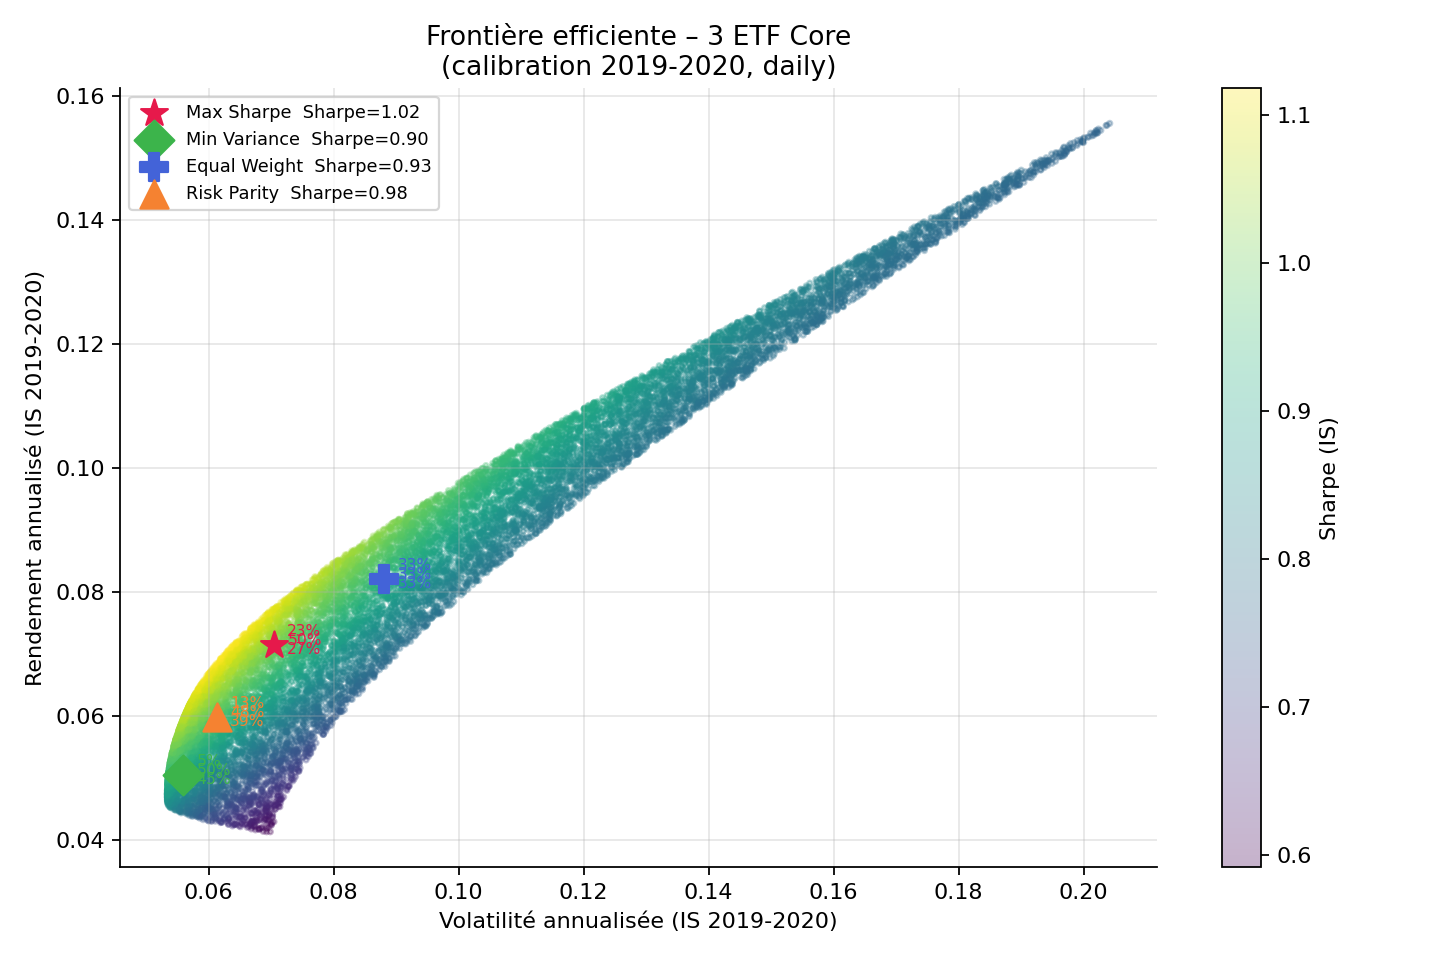
\includegraphics[width=0.9\textwidth]{06_efficient_frontier_core.png}
    \caption{Frontière efficiente des 3 ETF Core (2019--2020).}
\end{figure}

\begin{figure}[ht]
    \centering
    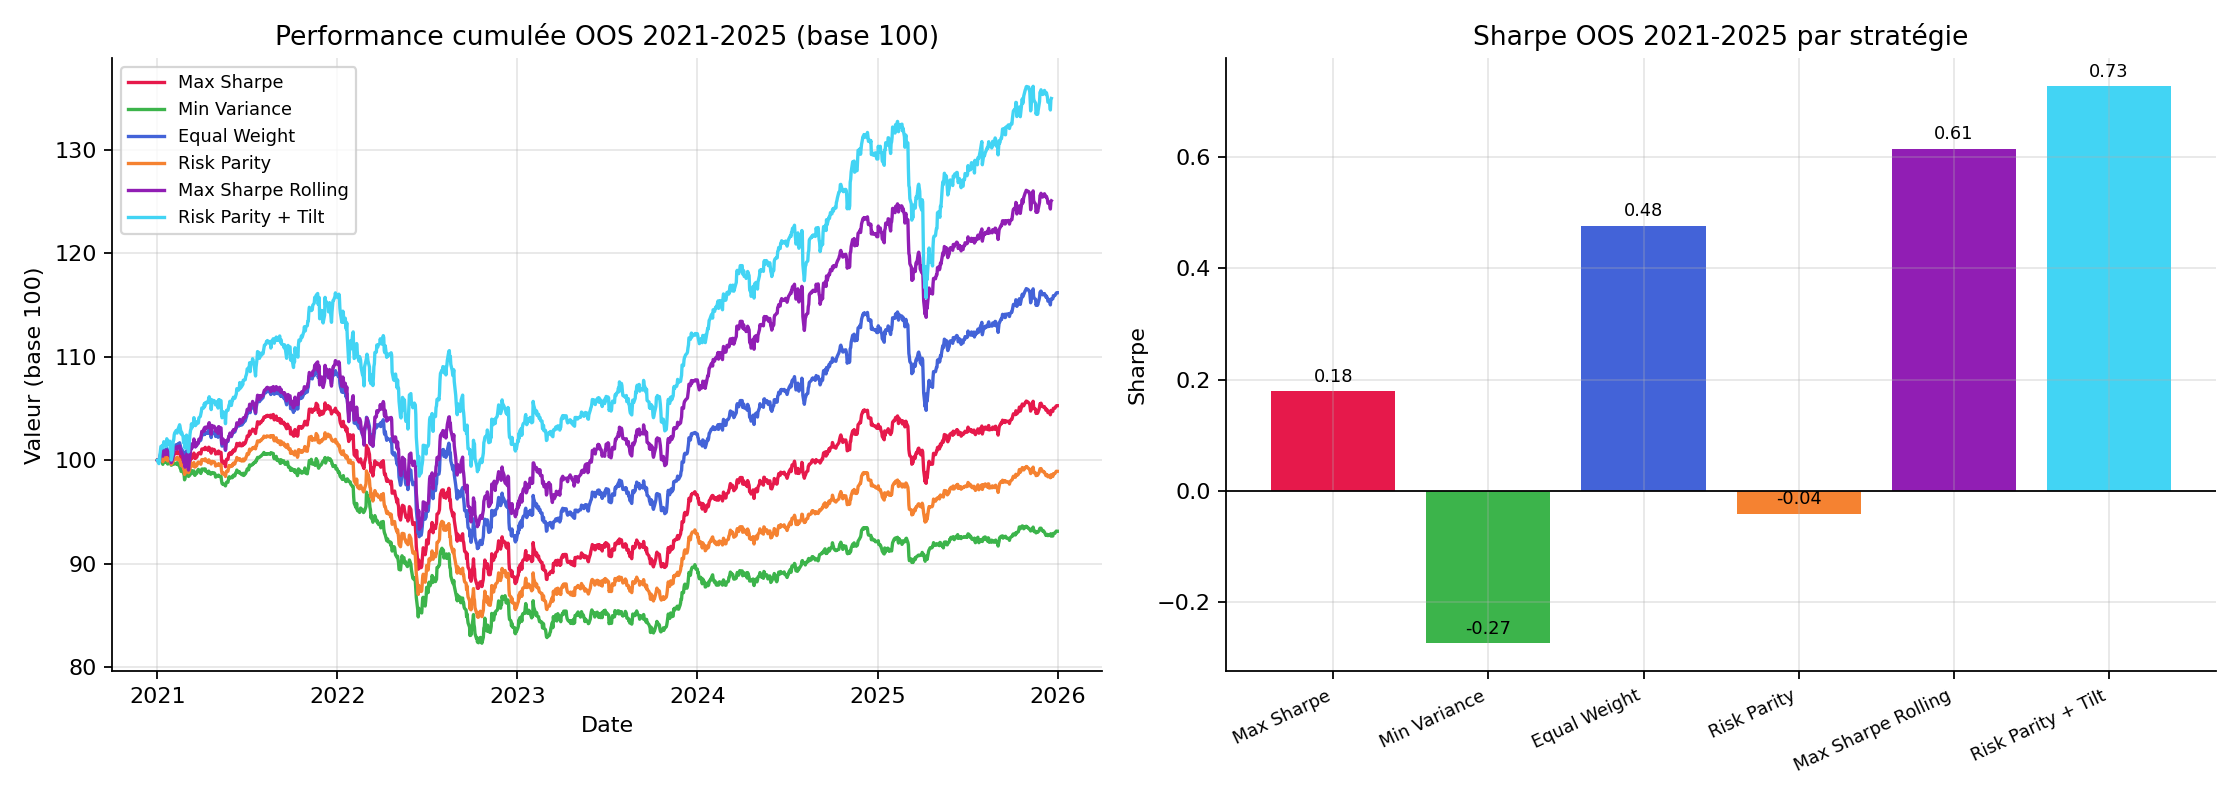
\includegraphics[width=0.9\textwidth]{07_core_strategies_oos_perf.png}
    \caption{Comparaison OOS des stratégies de pondération du Core.}
\end{figure}

\begin{figure}[ht]
    \centering
    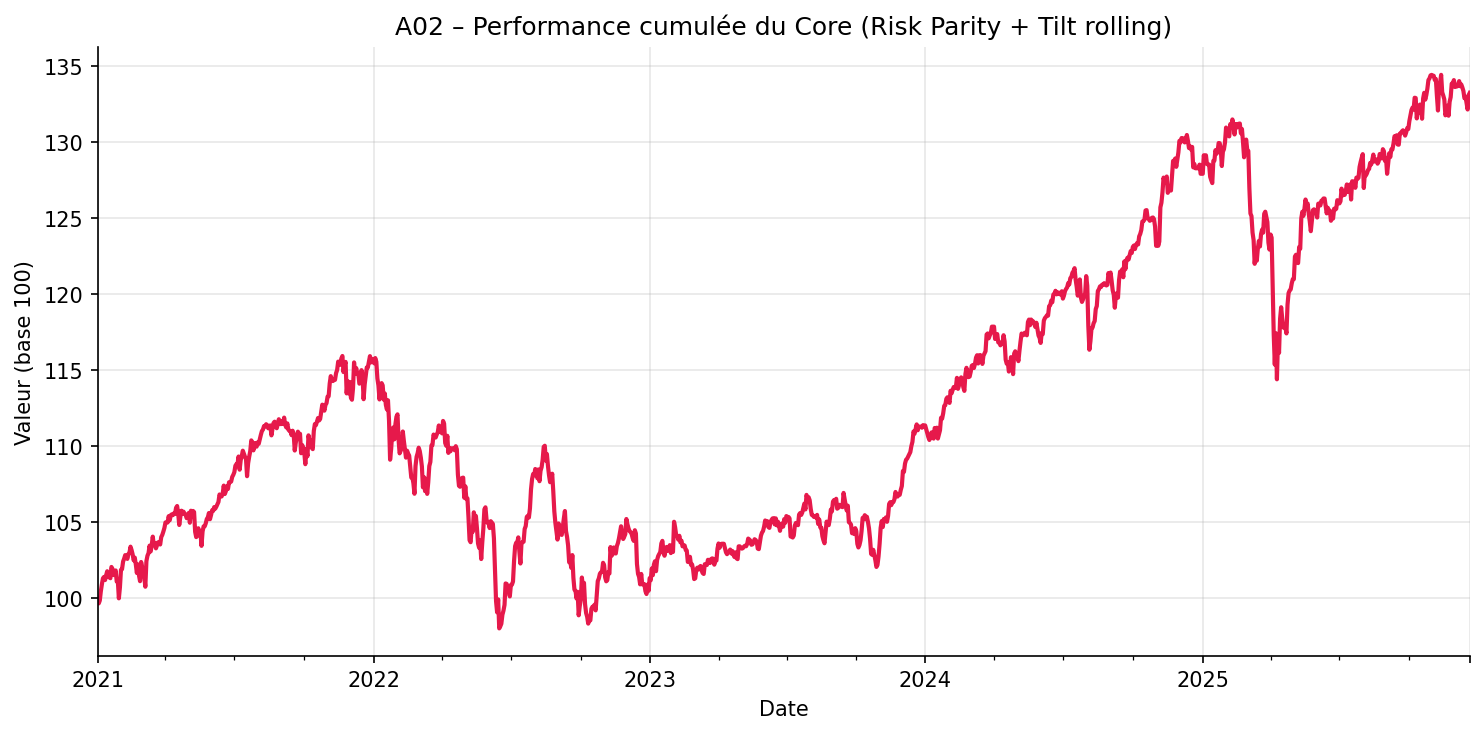
\includegraphics[width=0.9\textwidth]{A02_core_portfolio_cum.png}
    \caption{Performance cumulée du Core (logique Risk Parity + Tilt).}
\end{figure}

\begin{figure}[ht]
    \centering
    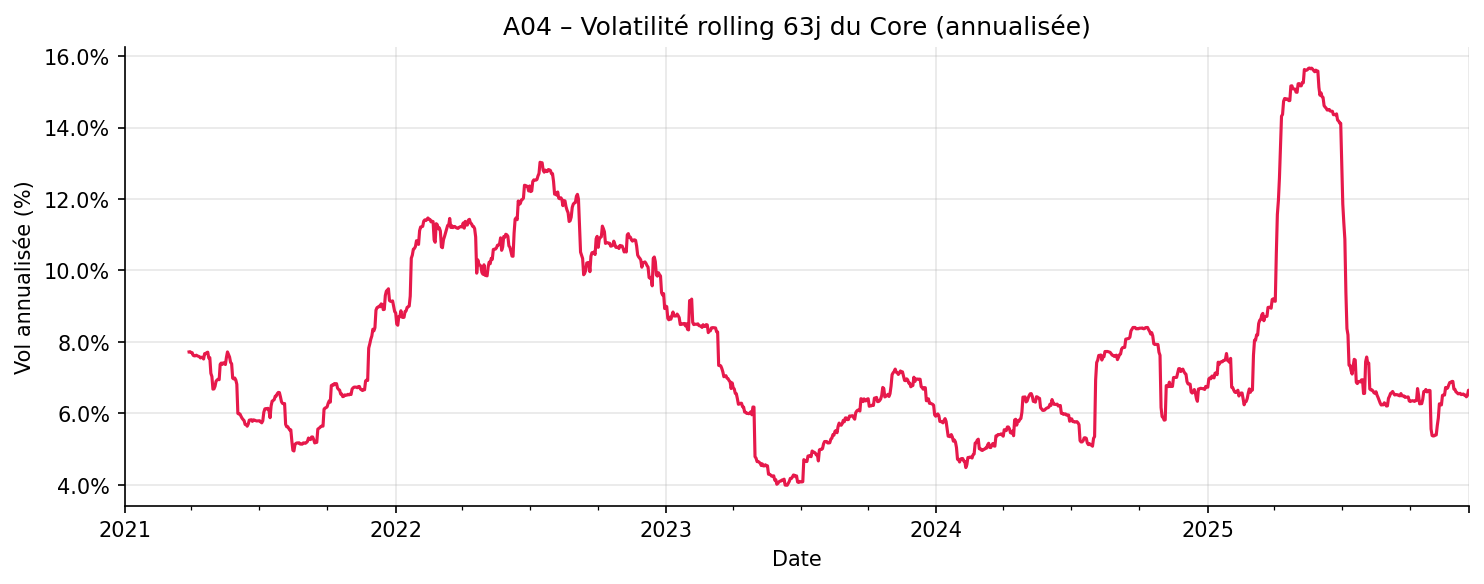
\includegraphics[width=0.9\textwidth]{A04_core_rolling_vol.png}
    \caption{Volatilité rolling 63 jours du Core.}
\end{figure}

\paragraph{Figure -- Frontière efficiente des 3 ETF Core}
Cette figure représente l’ensemble des portefeuilles réalisables à partir des trois ETF du Core sur la période de calibration 2019--2020. Chaque point correspond à une combinaison de poids différente entre l’ETF actions, l’ETF obligataire souverain et l’ETF crédit. L’axe horizontal mesure la volatilité annualisée et l’axe vertical le rendement annualisé. La couleur indique le niveau de Sharpe observé en calibration.

Cette représentation est utile car elle permet de situer les grandes familles de pondération par rapport à l’ensemble des allocations possibles. On observe que les portefeuilles très prudents se concentrent davantage sur les expositions obligataires, tandis que les portefeuilles plus risqués augmentent mécaniquement le poids de la poche actions. La frontière efficiente ne sert donc pas seulement à illustrer une optimisation théorique : elle permet de vérifier que notre univers Core est bien cohérent et qu’il offre un arbitrage rendement-risque exploitable.

\paragraph{Figure -- Comparaison OOS des stratégies Core}
Cette figure compare hors échantillon plusieurs modes de pondération du Core : Max Sharpe statique, Min Variance statique, Equal Weight, Risk Parity statique, Max Sharpe Rolling et Risk Parity + Tilt. Le message principal est que les portefeuilles statiques optimisés sur la période de calibration apparaissent plus fragiles hors échantillon. En particulier, Max Sharpe statique et Min Variance statique affichent des Sharpe OOS sensiblement inférieurs aux approches dynamiques.

À l’inverse, les méthodes rolling se montrent plus robustes, et la stratégie \textit{Risk Parity + Tilt} obtient le meilleur Sharpe OOS. Cela justifie le fait de ne pas retenir une pondération purement statique du Core. Notre choix final repose donc sur une logique de robustesse hors échantillon plutôt que sur la seule performance observée en calibration.

\paragraph{Figure A01 -- Performance cumulée des 3 ETF Core}
Cette figure présente l’évolution cumulée des trois ETF retenus dans le Core sur la période OOS 2021--2025. On constate que l’ETF actions constitue le principal moteur de performance, tandis que les poches souveraine et crédit ont évolué dans un contexte beaucoup moins favorable, marqué par la remontée des taux et la revalorisation du risque obligataire.

Ce constat n’est pas problématique en soi. Dans une allocation Core, chaque brique n’a pas vocation à maximiser isolément la performance, mais à apporter une source d’exposition spécifique. La poche actions apporte le potentiel de rendement, la poche obligataire souveraine joue un rôle d’amortisseur, et la poche crédit constitue une exposition intermédiaire. L’intérêt du Core se juge donc au niveau du portefeuille global, et non à partir de la seule performance individuelle de chacune des briques.

\paragraph{Figure A02 -- Performance cumulée du Core}
Cette figure montre la performance cumulée du portefeuille Core retenu, construit selon une logique \textit{Risk Parity + Tilt} en rolling. L’évolution est globalement croissante sur l’ensemble de la période, malgré plusieurs épisodes de stress marqués, notamment en 2022 puis lors des tensions observées en 2025.

Le principal intérêt de ce graphique est de montrer que la combinaison dynamique des trois ETF permet d’obtenir une trajectoire plus régulière qu’une exposition purement actions, tout en maintenant une capacité de participation à la hausse. Il s’agit donc d’un compromis entre performance et robustesse, cohérent avec le rôle structurel attendu de la poche Core.

\paragraph{Figure A03 -- Drawdown du portefeuille Core}
Cette figure représente le drawdown du Core, c’est-à-dire la perte relative par rapport au plus haut historique atteint jusque-là. Elle permet de visualiser la profondeur et la durée des phases de baisse.

On observe un drawdown maximal d’environ 15\%, ce qui reste cohérent avec une allocation diversifiée intégrant une poche actions dominante mais non exclusive. Ce graphique est important dans la mesure où il montre que l’intérêt du Core ne se limite pas au rendement annualisé : il réside aussi dans sa capacité à limiter les pertes extrêmes par rapport à une exposition plus concentrée.

\paragraph{Figure A04 -- Volatilité rolling 63 jours du Core}
La volatilité rolling 63 jours mesure la volatilité annualisée du portefeuille calculée sur les trois derniers mois de bourse environ. Cette figure ne montre donc pas la performance, mais le niveau de risque récent du Core à chaque date.

On observe une hausse nette de la volatilité en 2022, ce qui reflète logiquement le choc obligataire et les tensions macro-financières de la période. À l’inverse, les phases où la courbe redescend correspondent à des régimes de marché plus stables. Ce graphique est utile car il montre que le risque du Core n’est pas constant : il varie selon les conditions de marché. Cela justifie précisément l’intérêt d’une allocation dynamique et non d’une pondération figée une fois pour toutes.

\paragraph{Figure A05 -- Sharpe rolling 63 jours du Core}
Le Sharpe rolling 63 jours mesure, sur une fenêtre glissante de trois mois, le rendement ajusté du risque du portefeuille. Lorsque le ratio est positif et élevé, cela signifie que le portefeuille a récemment délivré une rémunération satisfaisante au regard de sa volatilité ; lorsqu’il devient négatif, cela traduit une dégradation conjoncturelle du couple rendement-risque.

Ce graphique complète utilement la volatilité rolling. En effet, une hausse de volatilité n’est pas nécessairement problématique si elle s’accompagne aussi d’un bon rendement. Le Sharpe rolling permet donc d’apprécier la qualité récente de la performance du Core, et de montrer que celle-ci varie selon les régimes de marché.

\paragraph{Figure A06 -- Performance annuelle du Core}
Cette figure synthétise les rendements annuels du Core. Elle met en évidence une année 2022 négative, suivie d’un redressement en 2023 et 2024, puis d’une performance plus modérée en 2025.

Cette lecture annuelle est importante car elle permet de replacer le comportement du Core dans le cycle de marché. Elle montre que le portefeuille n’est pas conçu pour éviter toute année négative, ce qui serait irréaliste sans levier défensif ou couverture spécifique, mais pour offrir une trajectoire globalement robuste et compatible avec un rôle de socle d’allocation.

\paragraph{Figure A07 -- Frais des ETF Core}
Cette figure présente les expense ratios des trois ETF composant le Core. Les niveaux observés restent faibles, ce qui est cohérent avec la philosophie même de la poche Core : obtenir une exposition liquide, transparente et peu coûteuse aux grands moteurs de marché.

Le faible niveau de frais constitue un point important de justification méthodologique. Dans une architecture Core-Satellite, la poche Core doit être peu coûteuse afin de préserver le budget de frais global et de laisser davantage de place à la poche Satellite, plus active et structurellement plus onéreuse. Le Core remplit donc bien ici son rôle d’exposition stratégique efficiente en coût.

\paragraph{Figure D01 -- Performance cumulée du portefeuille total vs Core}
Cette figure compare la performance cumulée du portefeuille Core-Satellite à celle du Core seul. On observe que la courbe du portefeuille total est légèrement inférieure à celle du Core sur une partie importante de la période.

Ce résultat n’est pas incohérent. La poche Satellite a été conçue avant tout comme une poche de diversification et de décorrélation, et non comme une poche destinée à surperformer systématiquement le Core en niveau absolu. Son rôle est d’améliorer le profil global du portefeuille, notamment en réduisant la dépendance à une seule source de risque. Il est donc tout à fait possible que le portefeuille final affiche un rendement légèrement inférieur au Core sur certaines périodes, tout en présentant un couple rendement-risque plus équilibré ou une meilleure robustesse dans les phases de stress.

Autrement dit, la comparaison pertinente ne doit pas porter uniquement sur la performance cumulée finale, mais aussi sur la volatilité, le drawdown, la corrélation entre poches et le respect des contraintes de frais et de diversification.

\section{Commentaires des graphiques de la poche Satellite et de l’interaction Core--Satellite}

\begin{figure}[ht]
    \centering
    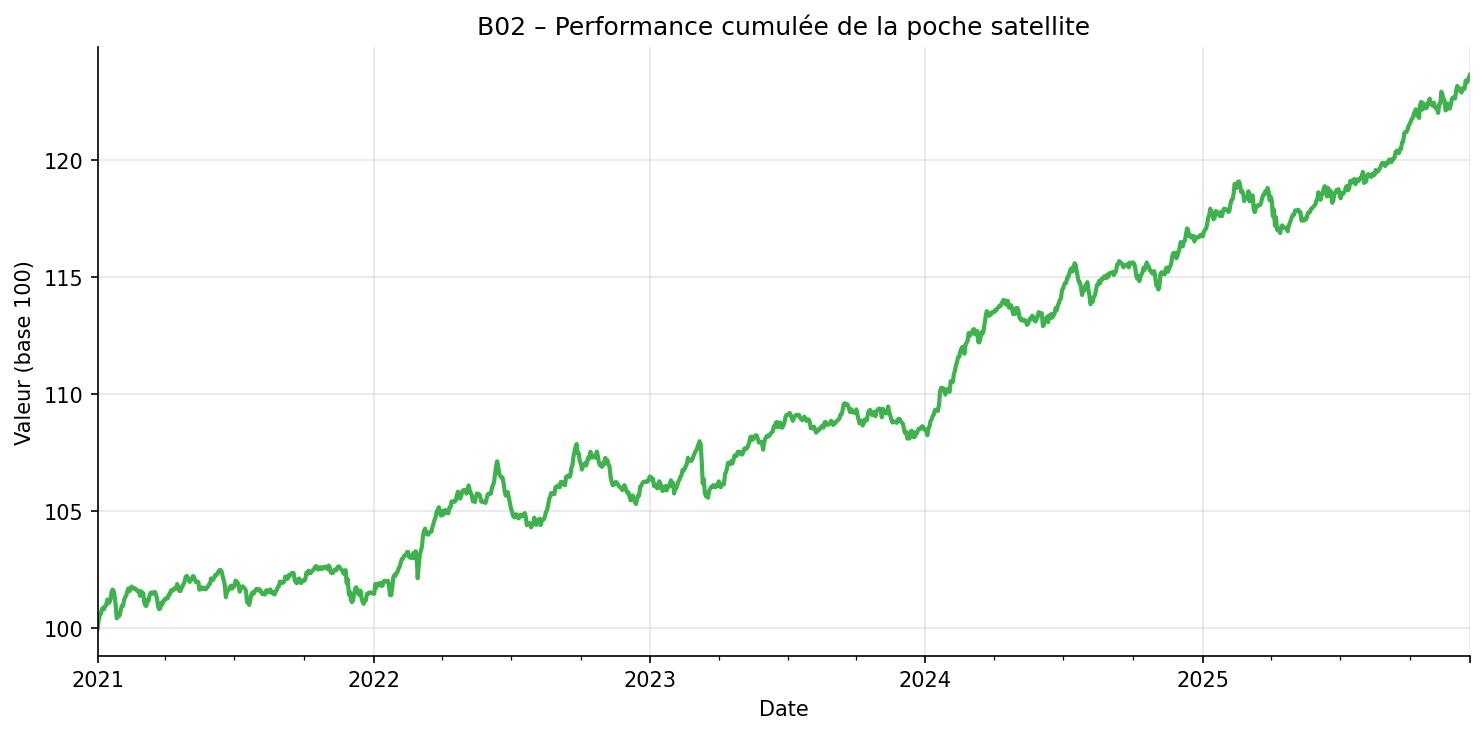
\includegraphics[width=0.9\textwidth]{B02_sat_pocket_cum.png}
    \caption{Performance cumulée de la poche Satellite agrégée.}
\end{figure}

\begin{figure}[ht]
    \centering
    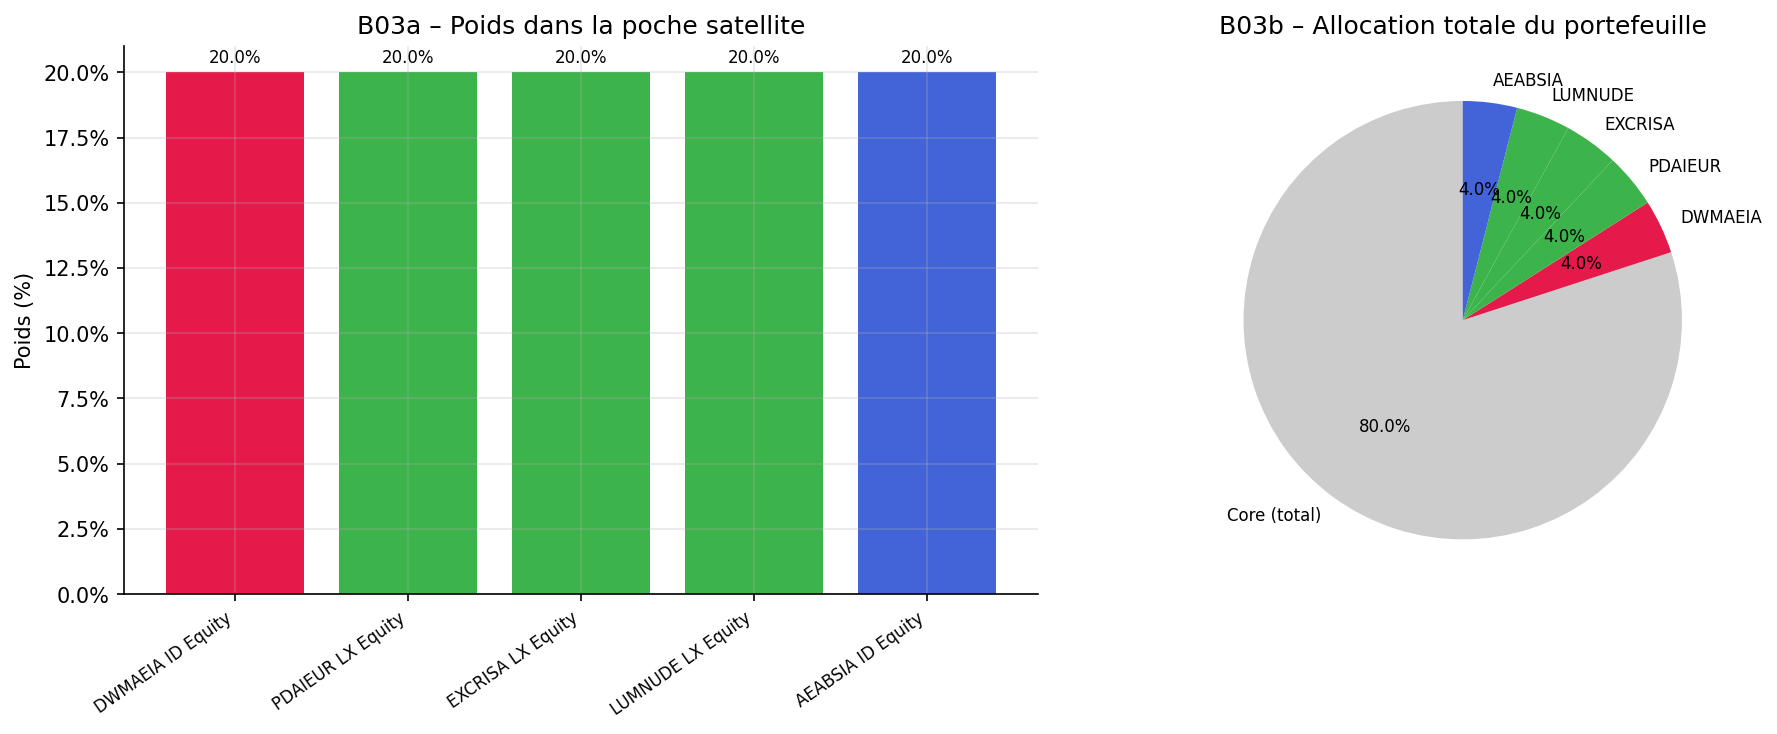
\includegraphics[width=0.9\textwidth]{B03_sat_weights.png}
    \caption{Poids intra-Satellite et allocation totale Core/Satellite.}
\end{figure}

\begin{figure}[ht]
    \centering
    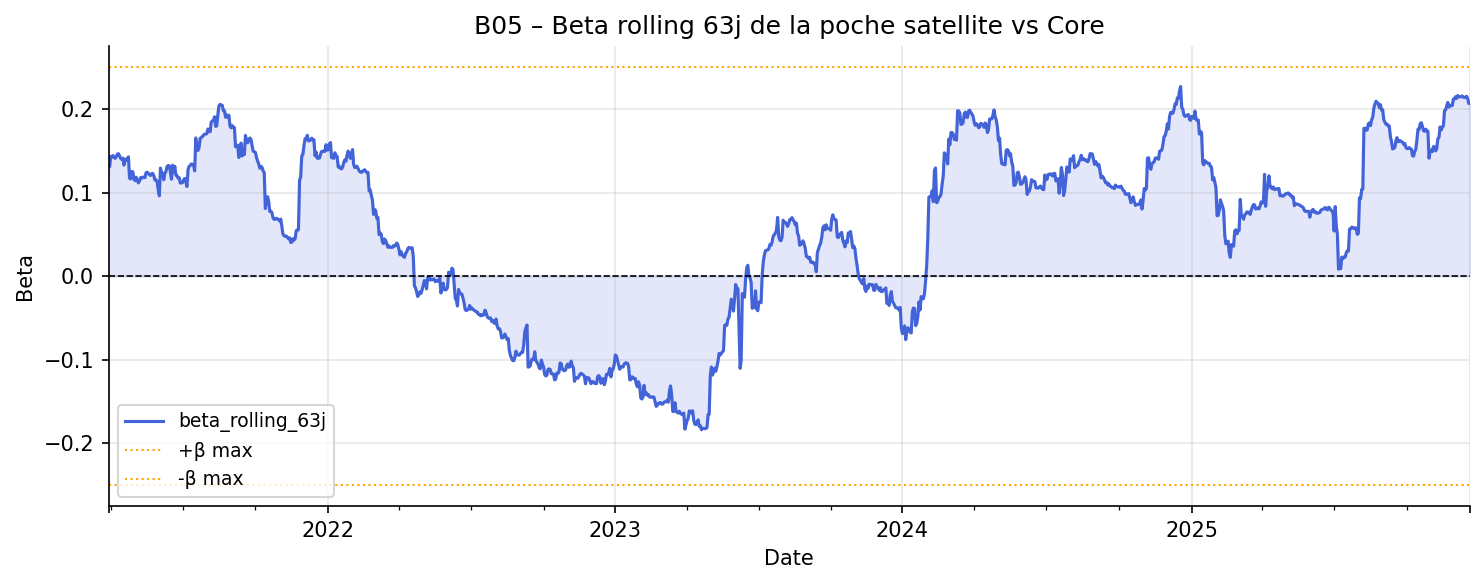
\includegraphics[width=0.9\textwidth]{B05_sat_rolling_beta.png}
    \caption{Bêta rolling 63 jours de la Satellite vs Core.}
\end{figure}

\begin{figure}[ht]
    \centering
    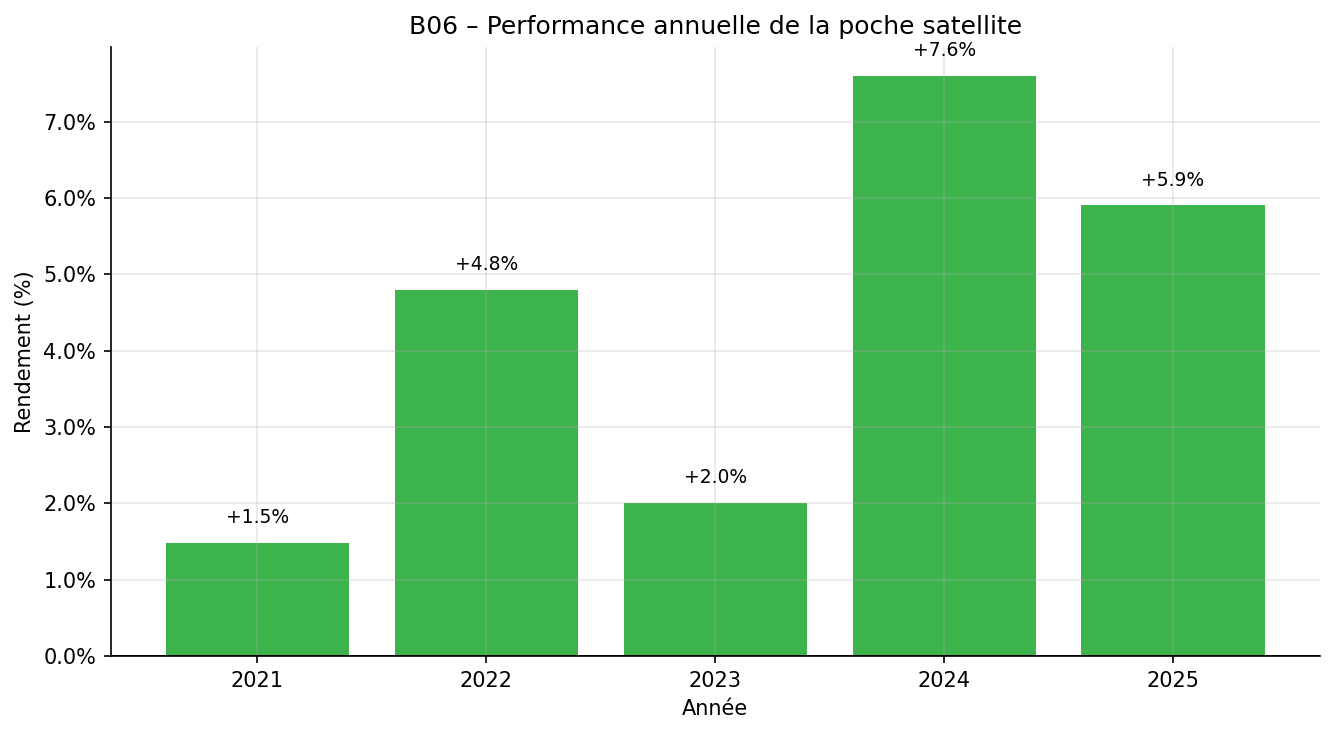
\includegraphics[width=0.9\textwidth]{B06_sat_annual.png}
    \caption{Performance annuelle de la Satellite.}
\end{figure}

\paragraph{Figure B01 -- Performance cumulée individuelle des fonds satellite}
Cette figure présente la performance cumulée de chacun des fonds retenus dans la poche Satellite sur la période OOS 2021--2025. Elle met en évidence une hétérogénéité importante des trajectoires individuelles, ce qui est attendu dans une poche satellite construite à partir de stratégies alternatives ou faiblement directionnelles.

Deux enseignements ressortent. Premièrement, les fonds ne suivent pas tous la même dynamique : certains affichent une progression plus régulière, tandis que d’autres connaissent des phases de stagnation ou de reprise plus tardive. Deuxièmement, cette dispersion est précisément ce qui rend l’agrégation intéressante. La poche Satellite n’a pas été pensée comme une juxtaposition de fonds tous similaires, mais comme un ensemble de briques complémentaires, issues de blocs différents, capables de réduire la concentration des risques.

\paragraph{Figure B02 -- Performance cumulée de la poche Satellite}
Cette figure montre la performance cumulée de la poche Satellite agrégée. La trajectoire est globalement croissante, avec une volatilité sensiblement plus faible que celle du Core. Cela confirme que la poche Satellite remplit bien son rôle de diversification : elle contribue positivement à la performance globale sans reproduire le profil de risque du Core.

Le point important à souligner est que la poche Satellite n’est pas construite pour battre mécaniquement la poche Core en performance absolue chaque année. Son objectif principal est d’apporter une source de rendement plus régulière, peu dépendante des grands moteurs traditionnels de marché, et donc utile à l’échelle du portefeuille global.

\paragraph{Figure B03 -- Poids dans la poche Satellite et allocation totale}
La première partie de la figure montre les poids des fonds à l’intérieur de la poche Satellite. Dans la version finale retenue, chaque fonds reçoit un poids identique, soit 20\% de la poche satellite. Ce choix d’équipondération repose sur une logique de simplicité, de lisibilité et de robustesse : il évite de surinterpréter les différences de scores estimées sur une période courte de calibration et limite le risque de concentration excessive sur un seul fonds.

La seconde partie de la figure montre l’allocation totale du portefeuille. On observe que la poche Core représente 80\% du portefeuille et la poche Satellite 20\%. Chaque fonds satellite ne représente donc que 4\% du portefeuille total. Cette structure est cohérente avec notre philosophie : une poche Core dominante, liquide et peu coûteuse, complétée par une poche Satellite plus spécialisée mais de taille maîtrisée.

\paragraph{Figure B04 -- Alpha rolling 63 jours de la poche Satellite vs Core}
Cette figure mesure l’alpha rolling annualisé de la poche Satellite relativement au Core, sur une fenêtre glissante de 63 jours. Lorsque la courbe est positive, cela signifie que la Satellite a récemment surperformé ce qui serait attendu compte tenu de son exposition au Core ; lorsqu’elle passe en territoire négatif, cela traduit une phase relative moins favorable.

Le graphique montre une alternance de phases positives et négatives, ce qui est normal sur une mesure rolling courte. L’enseignement principal est que l’alpha n’est pas structurellement négatif. Au contraire, la poche Satellite connaît plusieurs périodes de contribution relative positive, ce qui confirme qu’elle ne se contente pas d’être décorrélée : elle apporte aussi, par moments, une valeur ajoutée propre.

\paragraph{Figure B05 -- Beta rolling 63 jours de la poche Satellite vs Core}
Cette figure mesure le bêta rolling de la poche Satellite par rapport au Core. L’objectif visé dans la construction n’était pas un bêta strictement nul à chaque instant, ce qui serait irréaliste, mais un bêta globalement faible et contrôlé.

Le graphique montre que le bêta oscille autour de zéro sur l’ensemble de la période, avec des phases négatives puis positives. Cela confirme que la poche Satellite reste globalement peu directionnelle. En revanche, on observe aussi qu’en fin de période la courbe s’approche de la borne supérieure et la dépasse légèrement par moments. Ce point doit être assumé dans l’interprétation : la décorrélation reste présente, mais elle n’est pas parfaite ni constante. C’est précisément pour cette raison qu’il est plus rigoureux de parler d’une poche \emph{faiblement corrélée} ou \emph{modérément indépendante du Core}, plutôt que d’une couverture parfaite.

\paragraph{Figure B06 -- Performance annuelle de la poche Satellite}
Cette figure présente les rendements annuels de la poche Satellite. On constate que la poche Satellite est positive sur chacune des années observées, avec une contribution particulièrement marquée en 2022 et 2024.

Ce résultat est intéressant car il souligne le caractère stabilisateur de la Satellite. En particulier, en 2022, année difficile pour les expositions traditionnelles, la poche Satellite reste positive. Cela confirme qu’elle joue bien un rôle de diversification inter-régimes, c’est-à-dire qu’elle peut rester contributive même lorsque le cœur du portefeuille traverse une phase défavorable.

\paragraph{Figure B07 -- Frais des fonds Satellite}
Cette figure distingue, d’une part, les frais propres à chaque fonds et, d’autre part, leur contribution aux frais de la poche Satellite après pondération. On observe une forte hétérogénéité des expense ratios : certains fonds sont relativement peu coûteux, tandis que d’autres présentent des frais sensiblement plus élevés.

Ce graphique est important car il montre que la sélection n’a pas été faite uniquement sur la performance ou la décorrélation. Les frais ont aussi été intégrés dans le raisonnement global. Même si certains fonds satellite sont chers pris individuellement, leur poids limité dans le portefeuille total permet de maintenir une enveloppe de frais agrégée compatible avec la contrainte du projet.

\paragraph{Figure C01 -- Performance cumulée : Core vs Satellite vs Portefeuille}
Cette figure compare les trajectoires cumulées du Core, de la Satellite et du portefeuille total. On observe que la courbe du portefeuille se situe logiquement entre celle du Core et celle de la Satellite, puisque le portefeuille combine les deux poches.

Le message principal est que l’introduction de la Satellite ne transforme pas le portefeuille en moteur de surperformance systématique par rapport au Core. En revanche, elle modifie son profil global, en apportant une trajectoire plus diversifiée. Le portefeuille total apparaît ainsi comme un compromis entre la capacité de performance du Core et la régularité relative de la Satellite.

\paragraph{Figure C02 -- Rendements excédentaires cumulés du portefeuille par rapport au Core}
Cette figure mesure l’excès cumulé de performance du portefeuille total par rapport au Core seul. Une valeur positive signifie que le portefeuille surperforme le Core ; une valeur négative, qu’il le sous-performe.

Le graphique montre qu’après quelques phases de surperformance intermédiaires, le portefeuille termine en léger déficit relatif par rapport au Core. Ce résultat n’est pas incohérent avec notre construction. En effet, la poche Satellite a d’abord été intégrée comme outil de diversification, de stabilisation relative et de contrôle du profil de risque, et non comme une poche destinée à maximiser à tout prix l’excès de rendement. Ce point est essentiel à défendre : dans une architecture Core--Satellite, la réussite ne se juge pas uniquement à l’aune de la surperformance finale, mais aussi à la qualité du couple rendement-risque et à la robustesse de la construction.

\paragraph{Figure C04 -- Performance annuelle : Core vs Portefeuille vs Satellite}
Cette figure compare, année par année, les performances du Core, du portefeuille total et de la poche Satellite. Elle met bien en évidence la logique de combinaison entre les deux poches.

On observe notamment qu’en 2022 la Satellite joue un rôle amortisseur très clair, puisqu’elle reste positive alors que le Core est fortement négatif. À l’inverse, dans les années plus porteuses pour les actifs traditionnels, le Core domine davantage en performance. Le portefeuille total se situe alors dans une position intermédiaire, ce qui est cohérent avec une logique de diversification plutôt qu’avec une recherche de domination systématique d’une poche sur l’autre.

\paragraph{Figure C05 -- Rendement excédentaire annuel du portefeuille par rapport au Core}
Cette figure présente, pour chaque année, l’écart de rendement entre le portefeuille total et le Core. On constate que le portefeuille sous-performe le Core en 2021, 2023 et 2024, mais le surperforme en 2022 et légèrement en 2025.

Cette lecture annuelle est utile car elle nuance fortement l’interprétation de la performance cumulée finale. Elle montre que la Satellite a été particulièrement utile dans les phases de stress, en particulier en 2022, où elle améliore nettement le résultat relatif du portefeuille. En revanche, lorsque le régime de marché favorise fortement la poche actions du Core, l’introduction d’une Satellite plus prudente et plus décorrélée pèse mécaniquement sur la performance relative. Ce comportement est conforme à la logique de construction retenue.

\begin{figure}[ht]
    \centering
    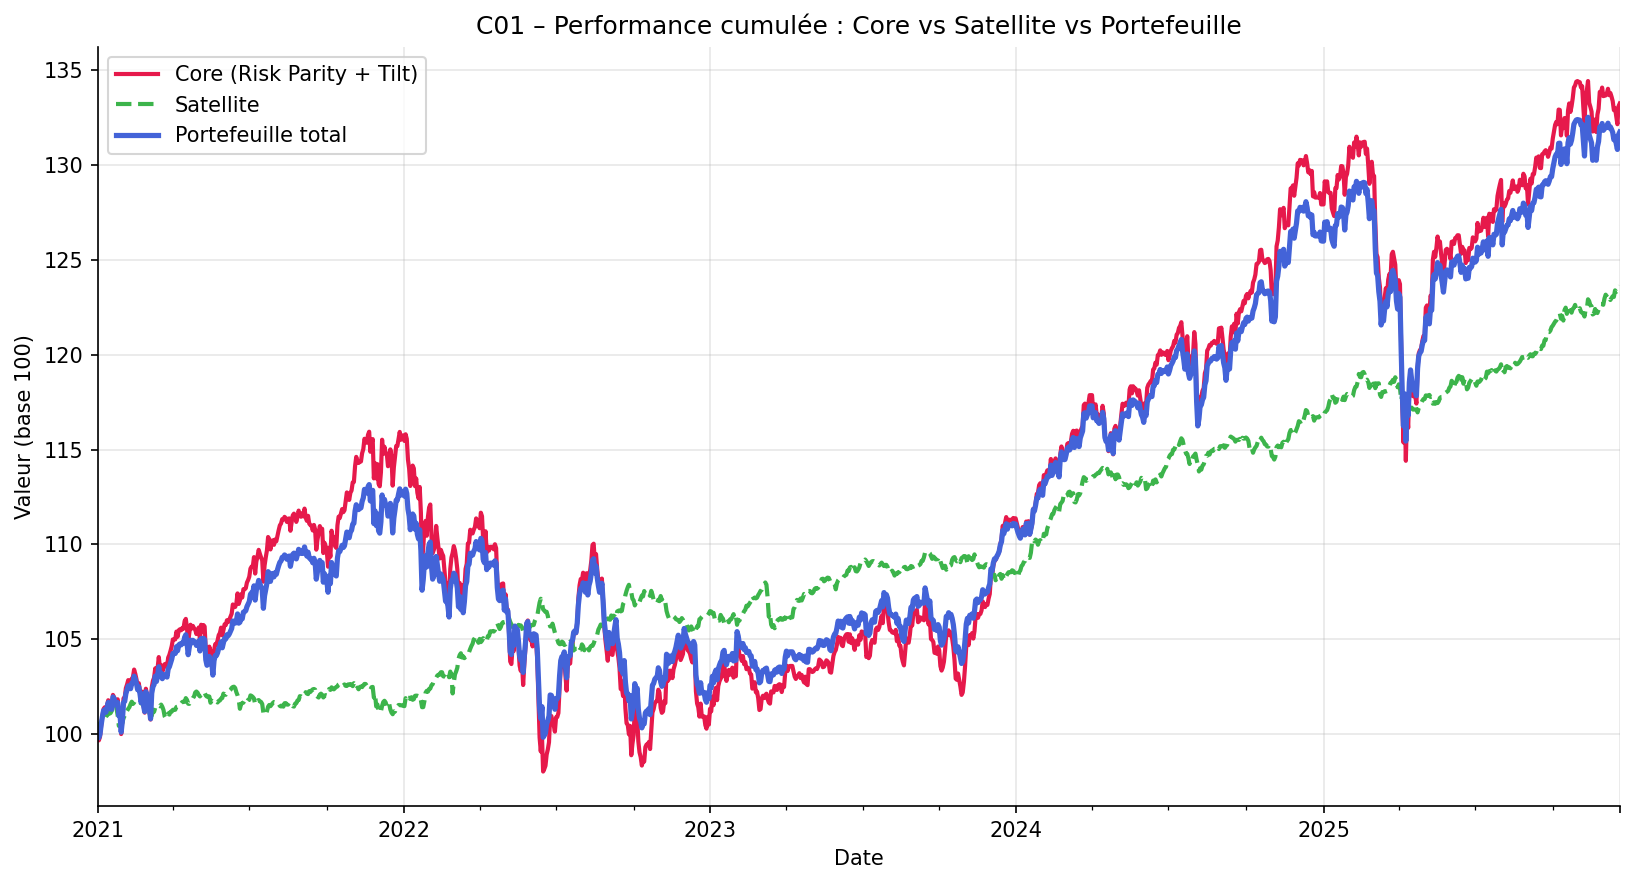
\includegraphics[width=0.9\textwidth]{C01_core_vs_sat_cum.png}
    \caption{Performance cumulée : Core vs Satellite vs Portefeuille total.}
\end{figure}

\begin{figure}[ht]
    \centering
    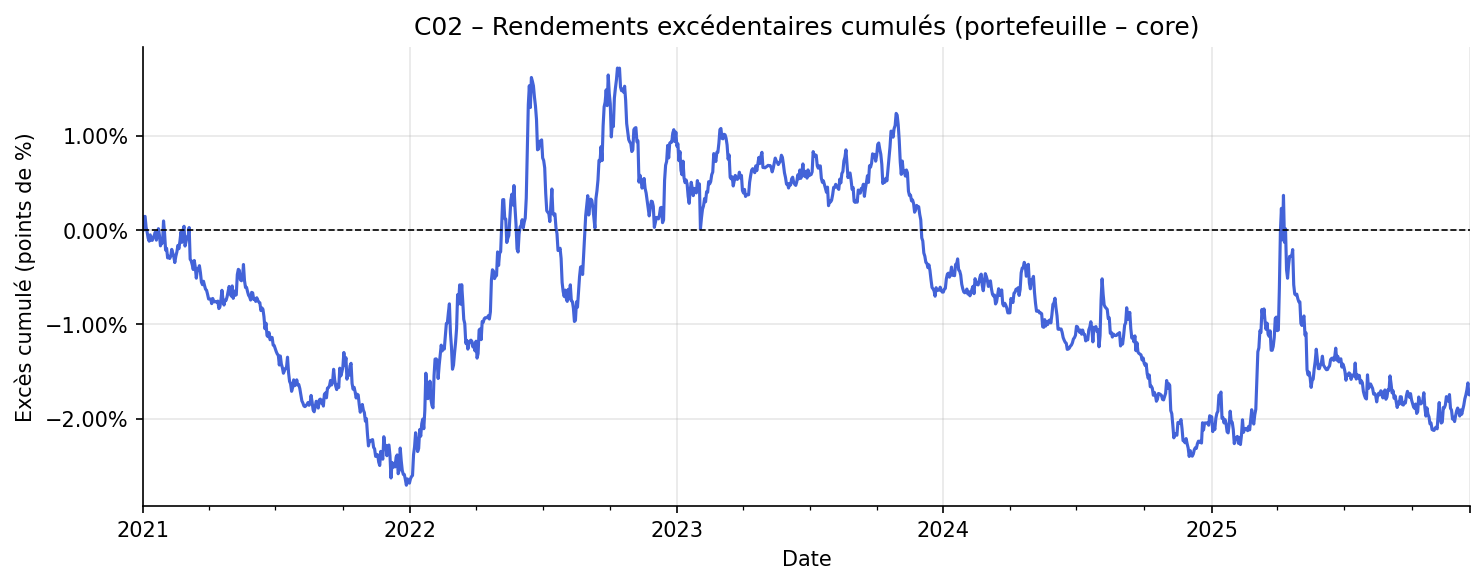
\includegraphics[width=0.9\textwidth]{C02_excess_cum.png}
    \caption{Rendements excédentaires cumulés du portefeuille vs Core.}
\end{figure}

\begin{figure}[ht]
    \centering
    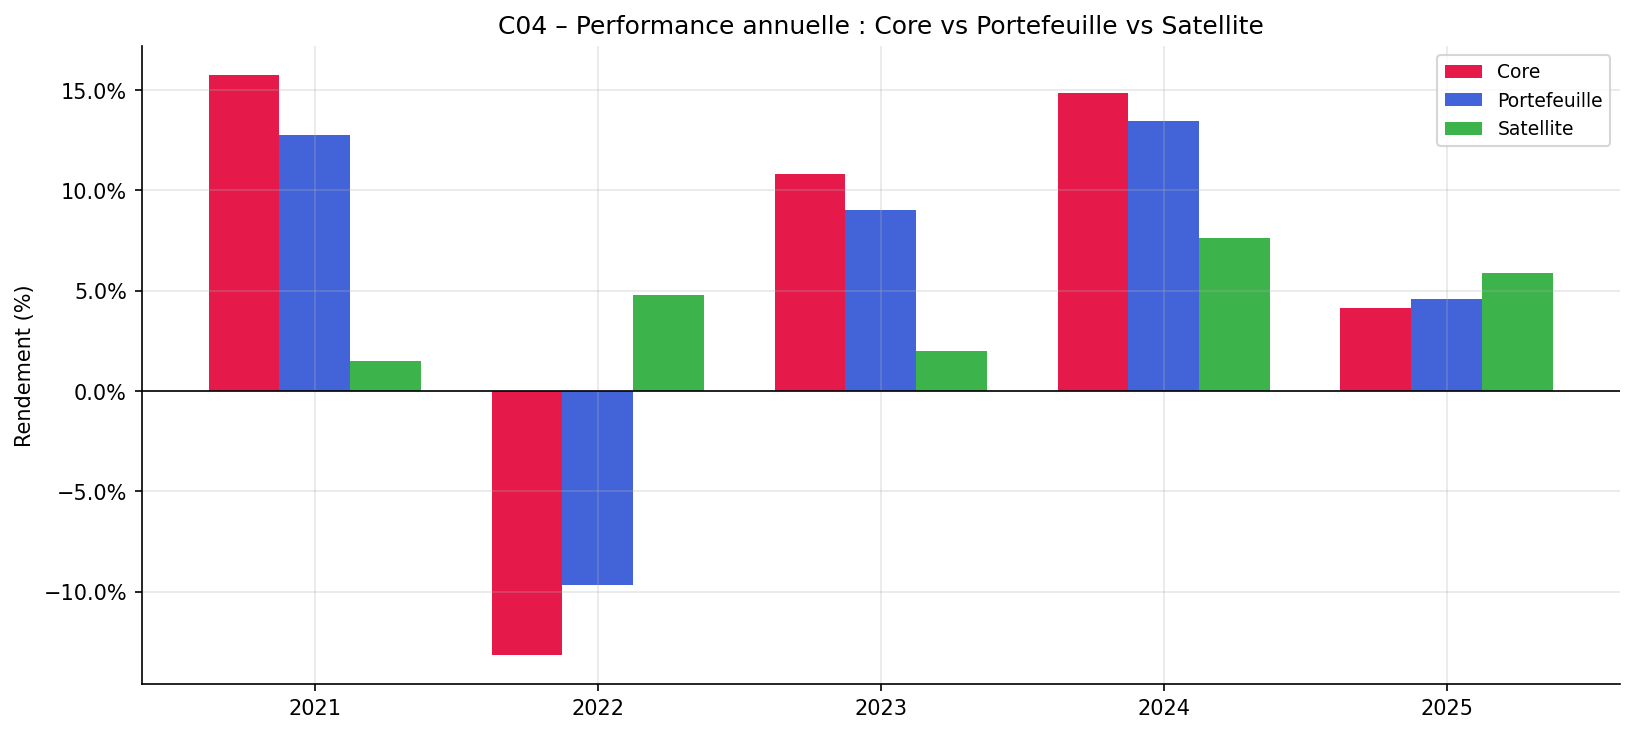
\includegraphics[width=0.9\textwidth]{C04_annual_grouped_bar.png}
    \caption{Performance annuelle : Core vs Portefeuille vs Satellite.}
\end{figure}

\begin{figure}[ht]
    \centering
    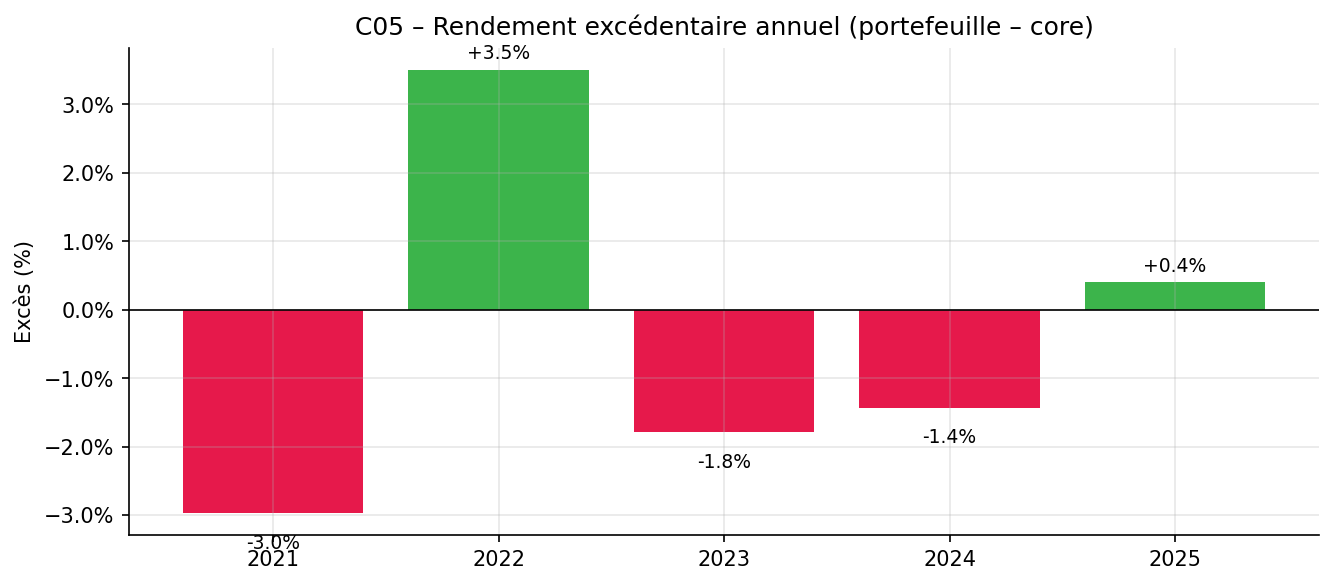
\includegraphics[width=0.9\textwidth]{C05_excess_annual.png}
    \caption{Rendement excédentaire annuel du portefeuille vs Core.}
\end{figure}

\section{Commentaires des graphiques du portefeuille total}

\begin{figure}[ht]
    \centering
    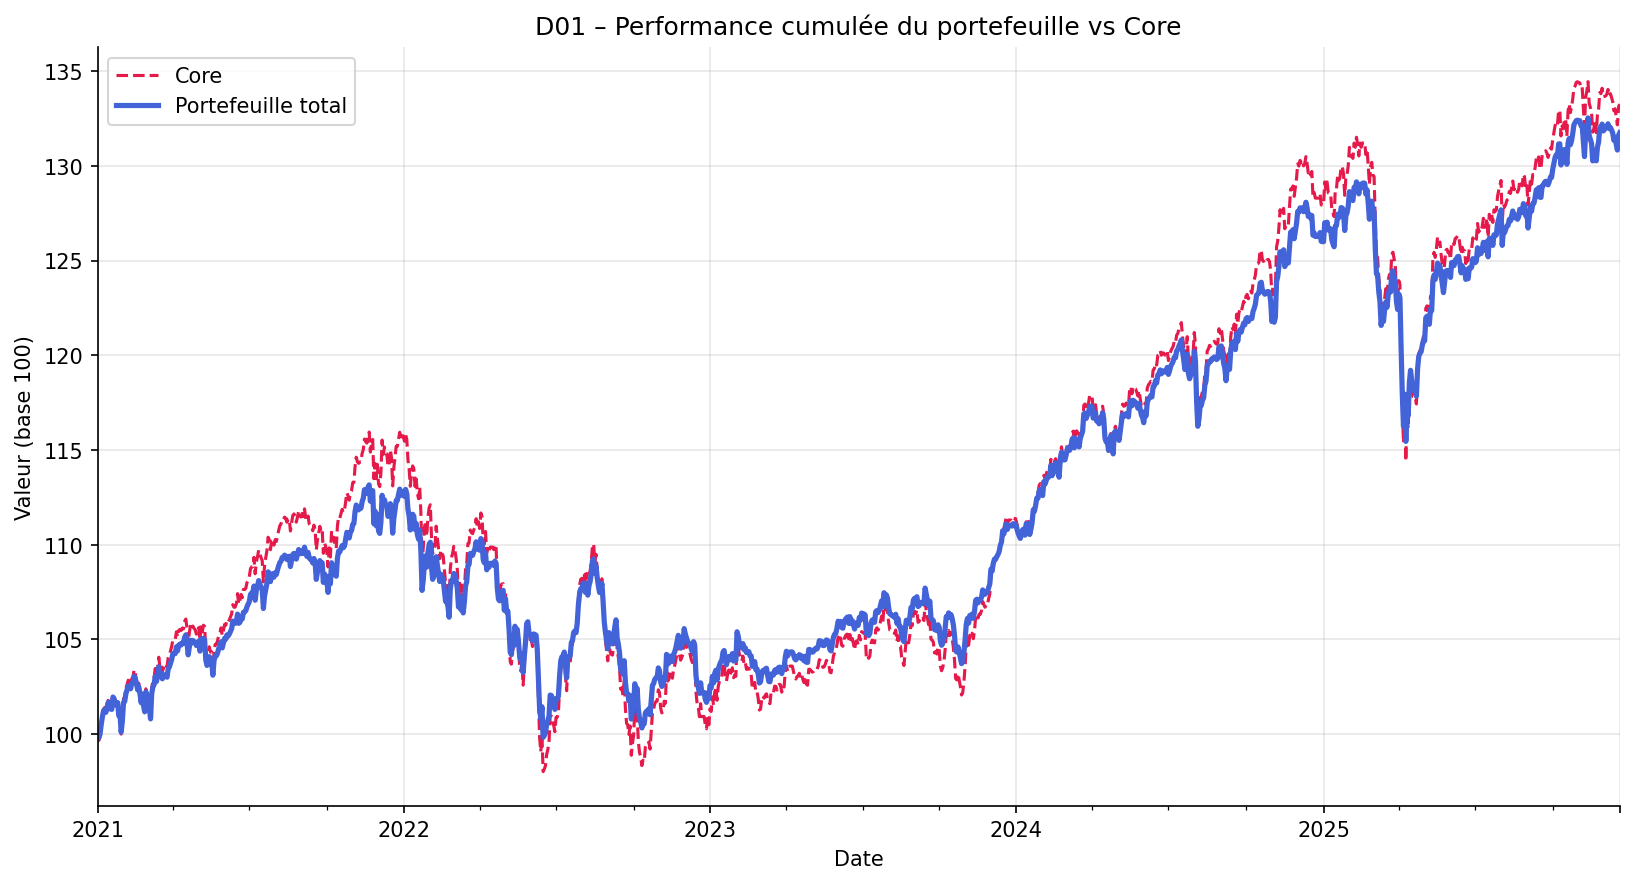
\includegraphics[width=0.9\textwidth]{D01_portfolio_cum.png}
    \caption{Performance cumulée du portefeuille vs Core.}
\end{figure}

\begin{figure}[ht]
    \centering
    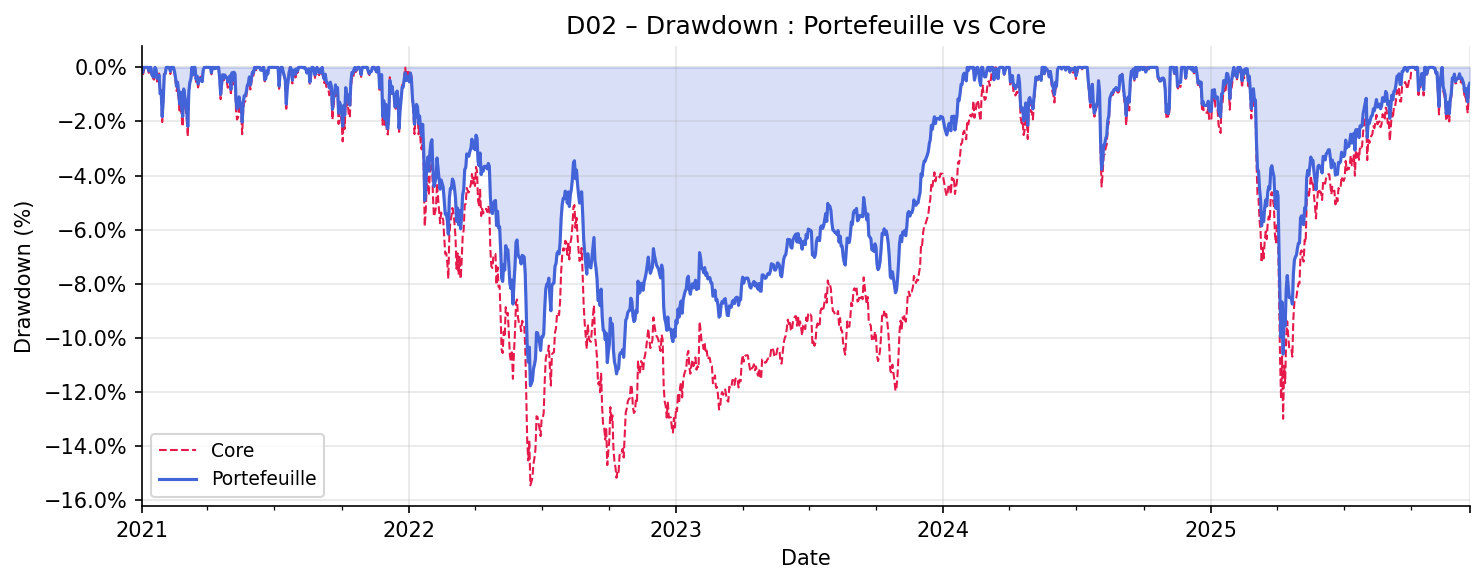
\includegraphics[width=0.9\textwidth]{D02_portfolio_drawdown.png}
    \caption{Drawdown du portefeuille vs Core.}
\end{figure}

\begin{figure}[ht]
    \centering
    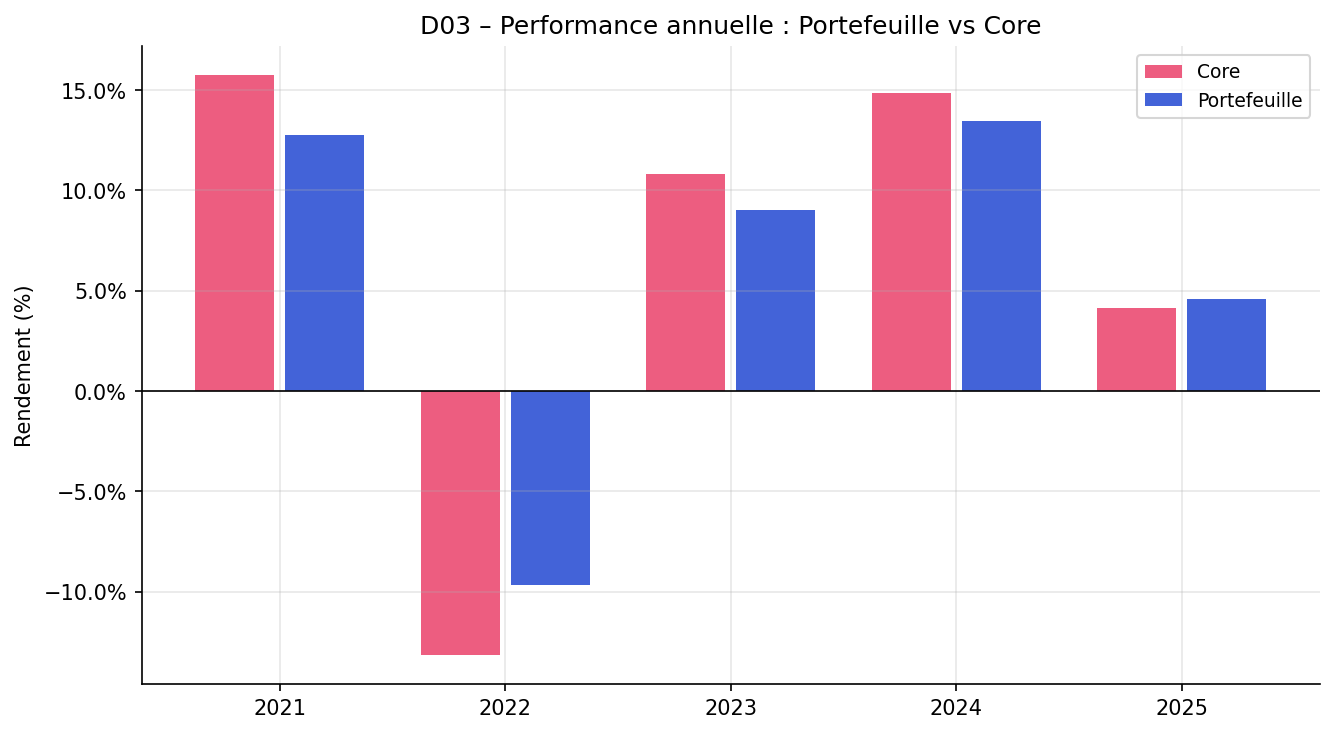
\includegraphics[width=0.9\textwidth]{D03_portfolio_annual.png}
    \caption{Performance annuelle : Portefeuille vs Core.}
\end{figure}

\begin{figure}[ht]
    \centering
    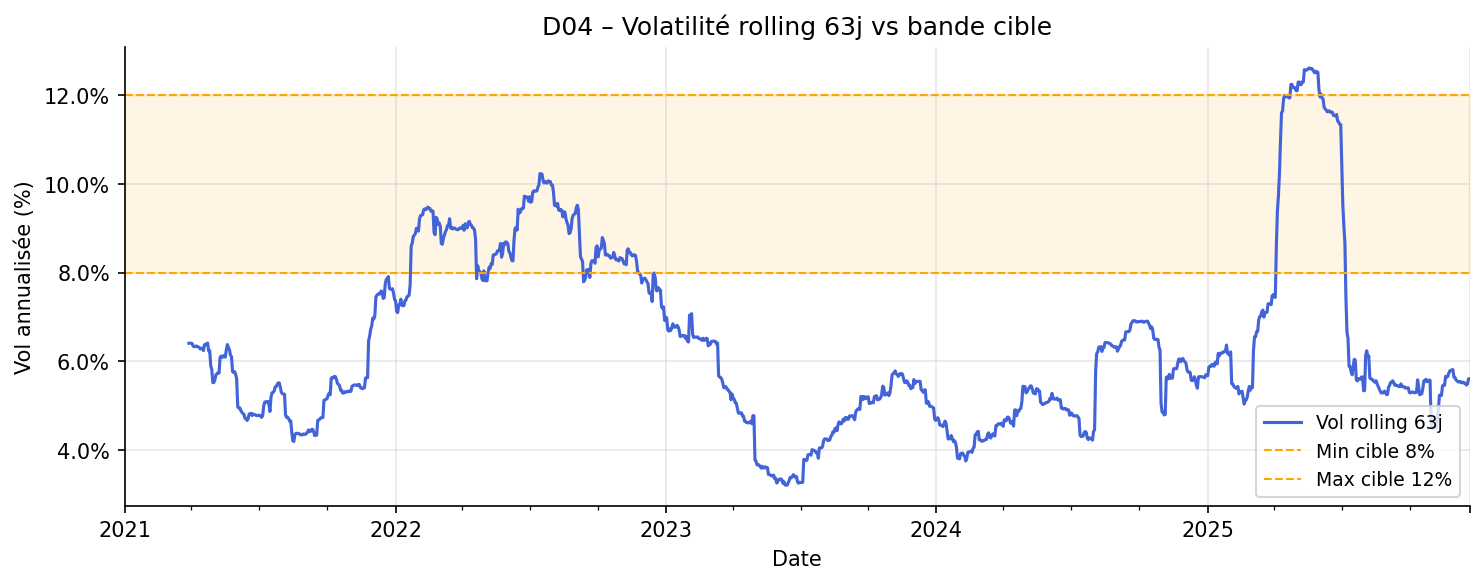
\includegraphics[width=0.9\textwidth]{D04_portfolio_vol_target.png}
    \caption{Volatilité rolling 63 jours du portefeuille vs bande cible 8--12\%.}
\end{figure}

\begin{figure}[ht]
    \centering
    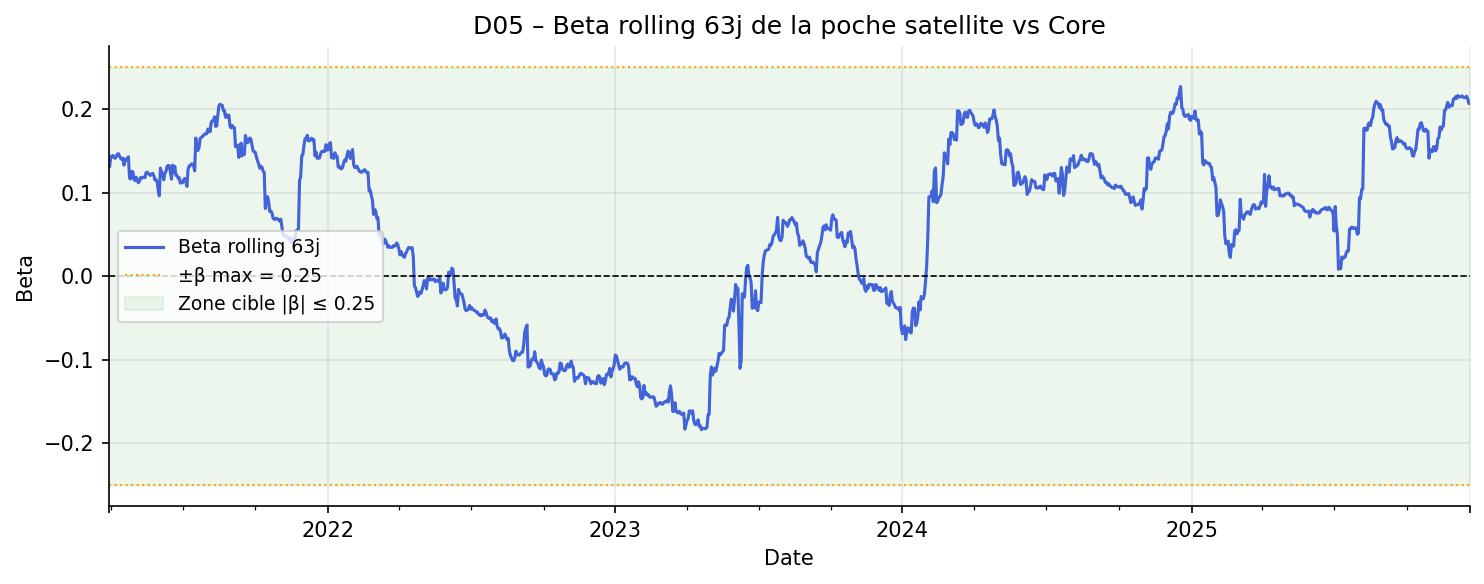
\includegraphics[width=0.9\textwidth]{D05_beta_sat_rolling.png}
    \caption{Bêta rolling 63 jours de la Satellite vs Core ($|\beta| \leq 0{,}25$).}
\end{figure}

\begin{figure}[ht]
    \centering
    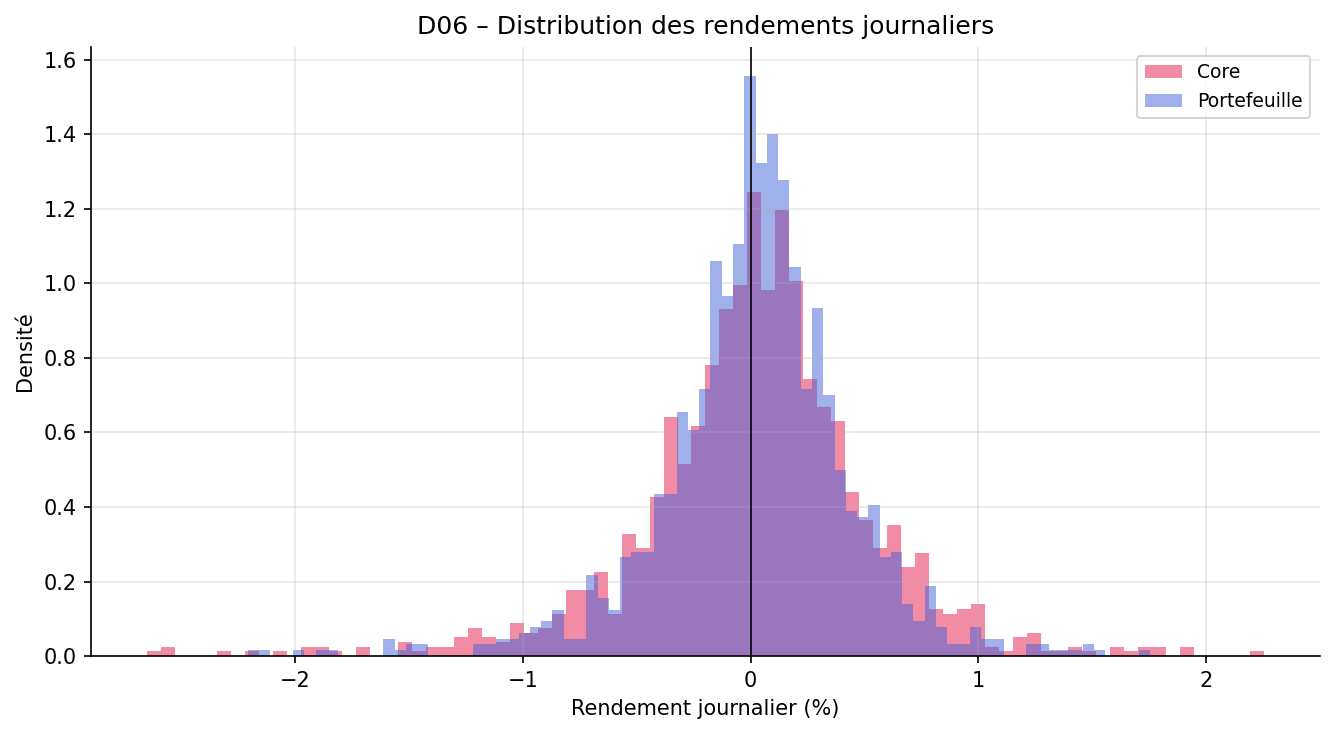
\includegraphics[width=0.9\textwidth]{D06_portfolio_dist.png}
    \caption{Distribution des rendements journaliers : portefeuille vs Core.}
\end{figure}

\paragraph{Figure D01 -- Performance cumulée du portefeuille vs Core}
Cette figure compare la performance cumulée du portefeuille total à celle du Core sur la période OOS 2021--2025. On observe que les deux trajectoires restent proches sur l’ensemble de la période, ce qui est logique puisque la poche Core demeure majoritaire dans l’allocation totale.

Le portefeuille total sous-performe légèrement le Core en performance cumulée finale. Ce résultat n’est pas incohérent avec la logique retenue. En effet, la poche Satellite n’a pas été introduite pour maximiser mécaniquement la performance absolue, mais pour améliorer la diversification, réduire la dépendance aux facteurs traditionnels de marché et amortir certaines phases défavorables. Le portefeuille total reflète donc un compromis : il conserve une forte exposition au moteur de performance du Core, tout en intégrant une poche plus défensive et plus décorrélée.

\paragraph{Figure D02 -- Drawdown : Portefeuille vs Core}
Cette figure compare les drawdowns du portefeuille total et du Core. On constate que les épisodes de baisse sont globalement moins profonds pour le portefeuille que pour le Core seul, en particulier durant certaines phases de stress comme 2022.

C’est un résultat important, car il montre que la poche Satellite a bien joué son rôle d’amortisseur. Même si elle n’a pas permis une surperformance systématique en niveau, elle a contribué à lisser le profil de risque du portefeuille. Cette lecture est essentielle dans une logique Core--Satellite : une bonne poche satellite ne doit pas nécessairement battre le Core à tout moment, mais elle doit améliorer la résilience globale du portefeuille.

\paragraph{Figure D03 -- Performance annuelle : Portefeuille vs Core}
Cette figure présente les rendements annuels du portefeuille total et du Core. Elle montre clairement que le portefeuille a moins bien performé que le Core en 2021, 2023 et 2024, mais qu’il a mieux résisté en 2022 et légèrement surperformé en 2025.

Cette hétérogénéité annuelle est cohérente avec la construction retenue. En régime de marché très favorable aux expositions traditionnelles, notamment actions, la présence d’une poche Satellite plus prudente freine mécaniquement la performance relative. En revanche, lorsque le contexte devient plus adverse, cette même poche peut amortir la baisse et améliorer le résultat relatif du portefeuille. La lecture de cette figure doit donc être faite conjointement avec celle des drawdowns et des performances excédentaires.

\paragraph{Figure D04 -- Volatilité rolling 63 jours du portefeuille vs bande cible}
Cette figure confronte la volatilité rolling annualisée du portefeuille à la bande cible de 8\% à 12\%. On observe que la volatilité réalisée se situe une grande partie du temps en dessous de la borne basse de 8\%, avec un bref dépassement au-dessus de 12\% en 2025.

Ce graphique est très utile pour l’interprétation du portefeuille final. Il montre que la structure retenue reste globalement trop prudente par rapport à l’objectif initial de risque. La principale explication est que la poche Satellite présente une volatilité très faible, de l’ordre de 2--3\% annualisés, et que son introduction réduit fortement la volatilité agrégée sans apporter suffisamment de risque additionnel pour maintenir le portefeuille dans la bande cible. Ce résultat n’invalide pas la construction, mais il montre que le portefeuille final est plus conservateur que prévu.

\paragraph{Figure D05 -- Beta rolling 63 jours de la poche Satellite vs Core}
Cette figure rappelle l’évolution du bêta rolling de la poche Satellite par rapport au Core, avec une zone cible définie par $|\beta| \leq 0{,}25$. Le bêta reste la plupart du temps dans cette zone, ce qui confirme que la poche Satellite demeure globalement peu directionnelle vis-à-vis du Core.

Ce graphique n’est pas à interpréter comme une mesure du risque du portefeuille total, mais comme une vérification structurelle de la mission assignée à la poche Satellite. Son intérêt est méthodologique : il montre que la Satellite n’a pas dérivé vers une poche trop corrélée ou trop exposée aux mêmes moteurs que le Core. Autrement dit, le portefeuille total reste bien construit comme une combinaison de deux poches distinctes, et non comme une duplication déguisée du Core.

\paragraph{Figure D06 -- Distribution des rendements journaliers}
Cette figure compare la distribution des rendements journaliers du portefeuille total à celle du Core. La distribution du portefeuille apparaît plus resserrée autour de zéro que celle du Core, avec des queues légèrement moins extrêmes.

Cela confirme visuellement ce que montraient déjà les indicateurs de volatilité et de drawdown : l’introduction de la poche Satellite réduit la dispersion des rendements quotidiens. En d’autres termes, le portefeuille total présente un profil de risque plus lissé, avec moins d’amplitude dans les variations journalières. Cette figure constitue donc une validation graphique de l’effet de diversification recherché.

\paragraph{Lecture d’ensemble des figures D}
Pris ensemble, les graphiques de la section D montrent que le portefeuille total n’a pas été conçu comme un simple portefeuille de surperformance face au Core. Il a été construit comme une combinaison visant à préserver une bonne capacité de performance tout en améliorant la robustesse du profil rendement--risque.

Le résultat final est cohérent avec cette logique : le portefeuille sous-performe légèrement le Core en performance cumulée, mais il présente un drawdown moins sévère, une distribution des rendements plus resserrée et une meilleure résistance dans les années difficiles. Le principal point d’attention reste la volatilité réalisée, qui demeure trop souvent inférieure à la cible de 8--12\%. Cela suggère que, dans une version ultérieure du projet, il pourrait être pertinent soit d’augmenter légèrement le risque de la poche Satellite, soit d’élargir la plage de pondération autorisée pour maintenir un niveau de risque plus proche de l’objectif initial, sans recourir au levier.

\subsubsection{Bénéfice de diversification selon le poids satellite}

\begin{figure}[ht]
    \centering
    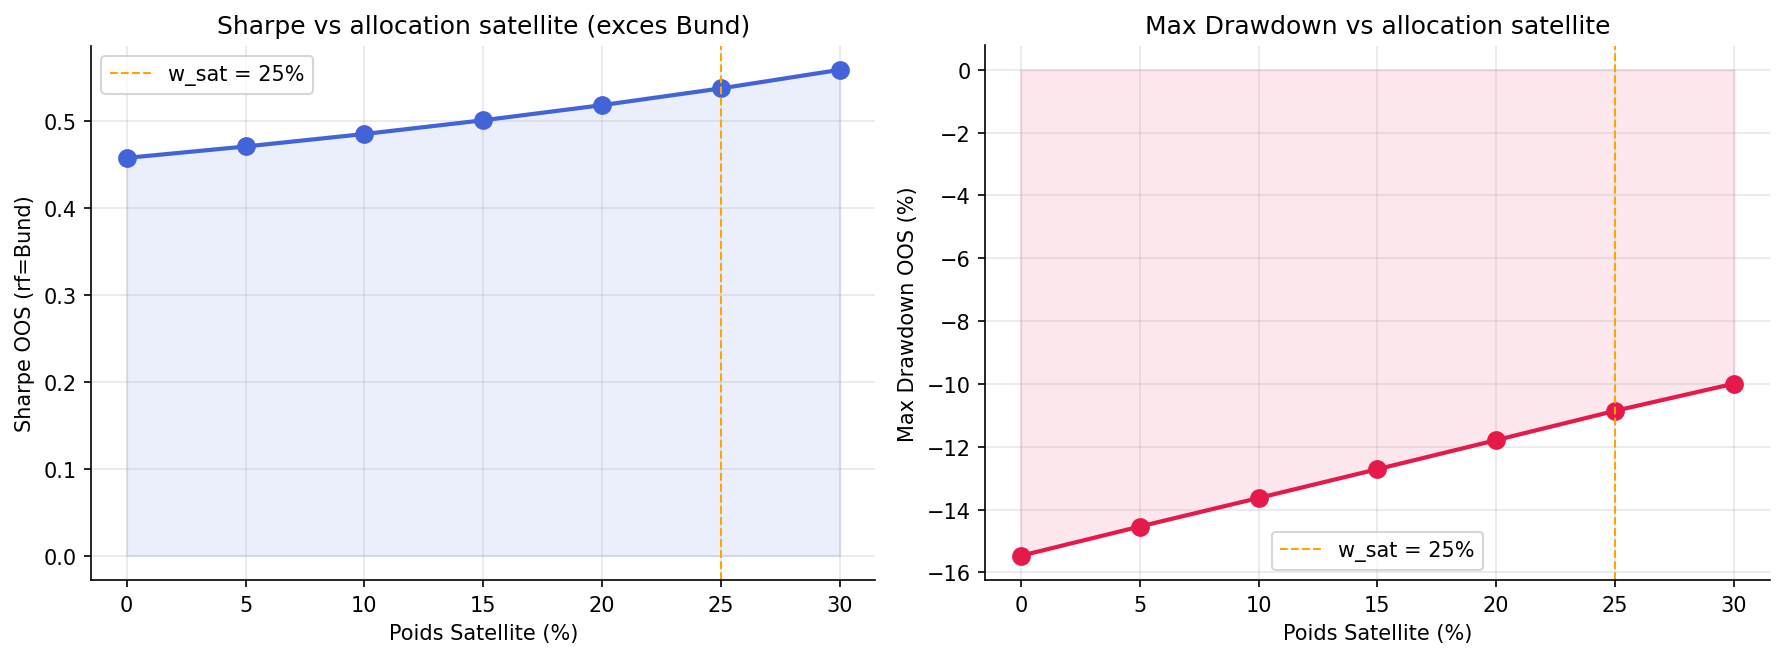
\includegraphics[width=0.9\textwidth]{E01_diversification_benefit.png}
    \caption{Bénéfice de diversification selon le poids satellite.}
\end{figure}

La figure montre l’effet d’une augmentation progressive du poids de la poche satellite dans le portefeuille global, de 0\% à 30\%.

Deux résultats ressortent clairement. D’une part, le ratio de Sharpe hors échantillon augmente de manière régulière lorsque la part satellite progresse. D’autre part, le maximum drawdown devient moins sévère à mesure que l’allocation satellite augmente. Autrement dit, dans notre backtest, l’introduction de la poche satellite améliore le couple rendement/risque du portefeuille et contribue à amortir les pertes extrêmes.

Ce résultat confirme que la poche satellite joue bien son rôle économique : elle n’est pas seulement une source potentielle d’alpha, elle constitue également un instrument de diversification au sein du portefeuille global. La ligne verticale placée à 25\% correspond au poids satellite retenu dans notre construction finale. Ce niveau apparaît comme un compromis prudent et cohérent : il permet déjà de capter une part importante du bénéfice de diversification tout en restant fidèle à l’esprit d’un portefeuille \textit{Core-Satellite}, dans lequel le Core demeure largement dominant.

Il faut toutefois noter que, sur les critères représentés ici, une allocation légèrement plus élevée aurait pu sembler encore plus favorable dans le backtest. Nous n’avons cependant pas cherché à maximiser mécaniquement ce résultat ponctuel, mais plutôt à retenir une allocation robuste, lisible et défendable dans le cadre du projet.

\subsubsection{Corrélation rolling entre la poche satellite et le Core}

\begin{figure}[ht]
    \centering
    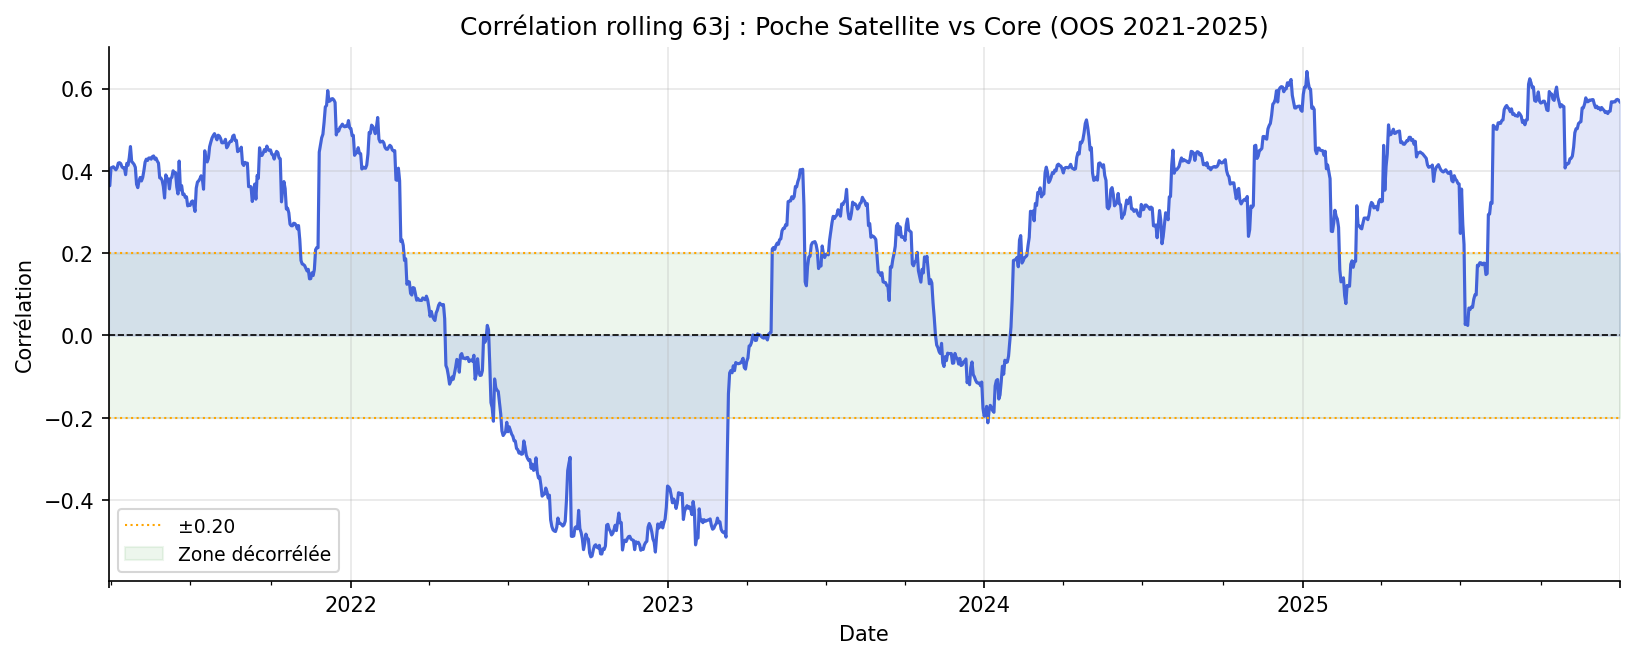
\includegraphics[width=0.9\textwidth]{E02_rolling_correlation.png}
    \caption{Corrélation rolling 63 jours entre Satellite et Core.}
\end{figure}

La corrélation glissante à 63 jours entre la poche satellite et le Core permet d’évaluer la stabilité temporelle de la diversification apportée par la poche satellite.

Le principal enseignement de cette figure est que la corrélation n’est pas constante dans le temps. Elle évolue sensiblement selon les phases de marché : elle devient parfois négative, ce qui traduit un véritable effet de couverture, mais elle peut aussi redevenir positive, voire dépasser temporairement la zone de faible corrélation. Cela signifie que la poche satellite n’est pas parfaitement décorrélée du Core à chaque instant.

Cette variabilité n’invalide toutefois pas la logique de construction retenue. En pratique, une poche satellite n’a pas besoin d’être en permanence dans une zone de corrélation strictement nulle ou négative pour être utile. Il suffit qu’elle présente, en moyenne, une sensibilité limitée au Core et qu’elle améliore effectivement le profil rendement/risque du portefeuille global. C’est précisément ce que montrent nos autres résultats : le bêta de la poche satellite reste modéré, la corrélation moyenne demeure contenue, et l’introduction du satellite améliore à la fois le Sharpe global et le drawdown.

Ainsi, cette figure doit être interprétée comme un indicateur de réalisme méthodologique : la décorrélation existe, mais elle n’est ni parfaite ni immuable. Notre conclusion n’est donc pas que la poche satellite est systématiquement indépendante du Core, mais qu’elle apporte une diversification suffisamment robuste pour justifier son intégration au portefeuille.

\section{Décomposition synthétique de la performance}

\begin{figure}[ht]
    \centering
    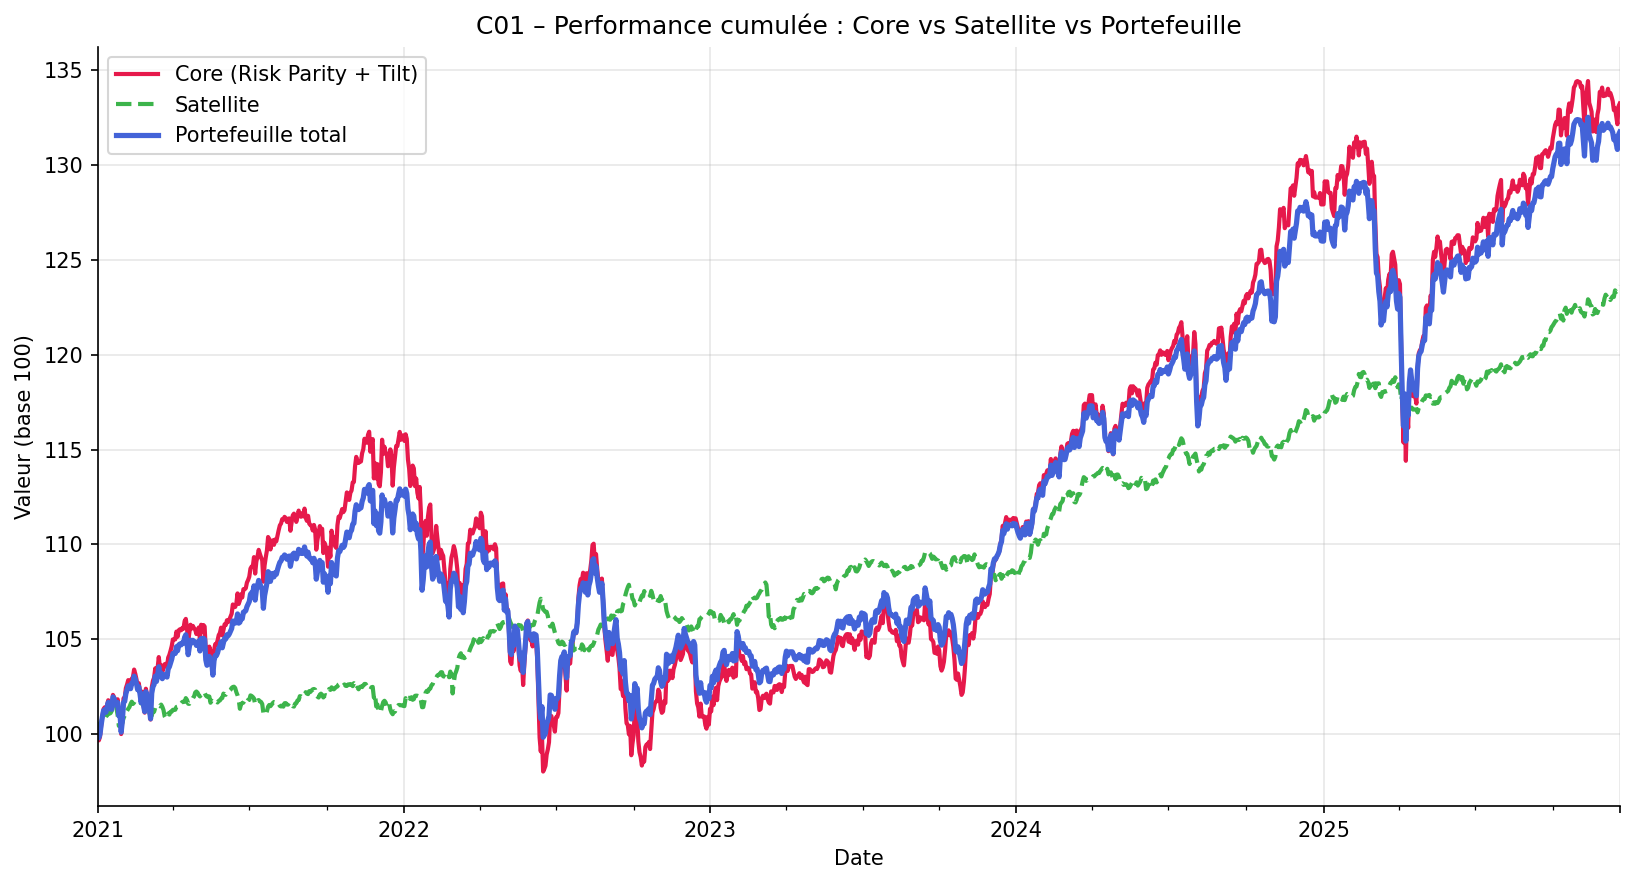
\includegraphics[width=0.9\textwidth]{C01_core_vs_sat_cum.png}
    \caption{Performance cumulée : Core vs Satellite vs Portefeuille total.}
\end{figure}

\begin{figure}[ht]
    \centering
    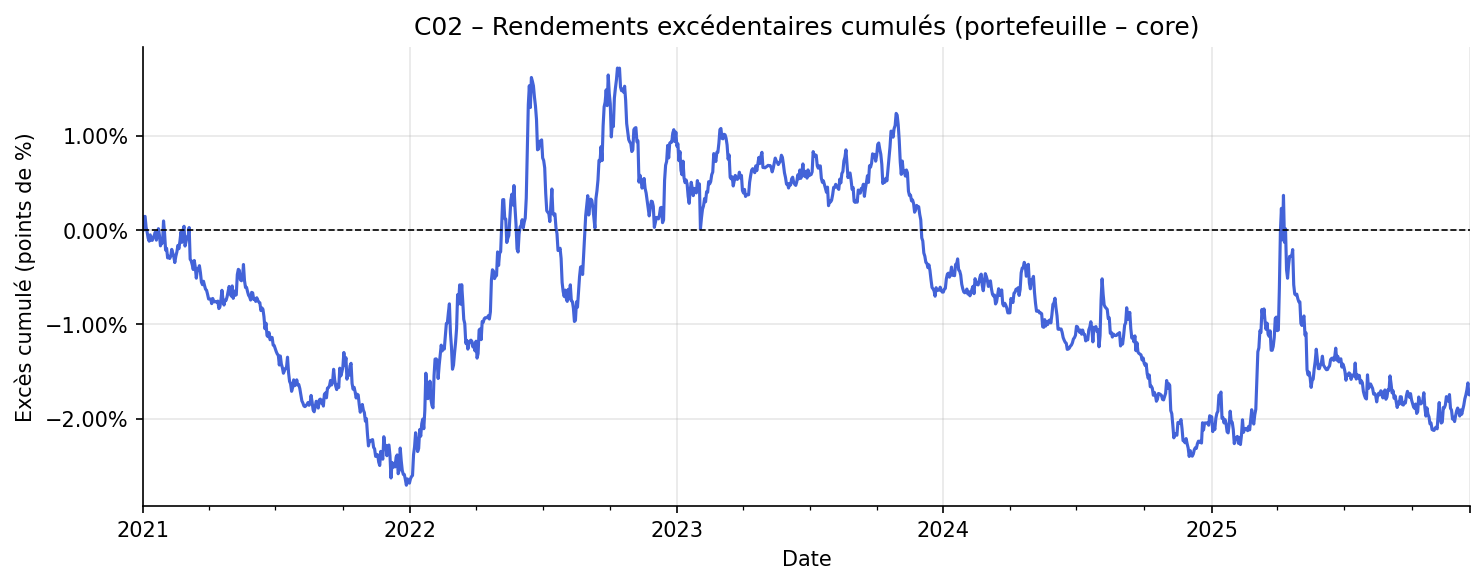
\includegraphics[width=0.9\textwidth]{C02_excess_cum.png}
    \caption{Excès de performance cumulée du portefeuille vs Core.}
\end{figure}

\begin{figure}[ht]
    \centering
    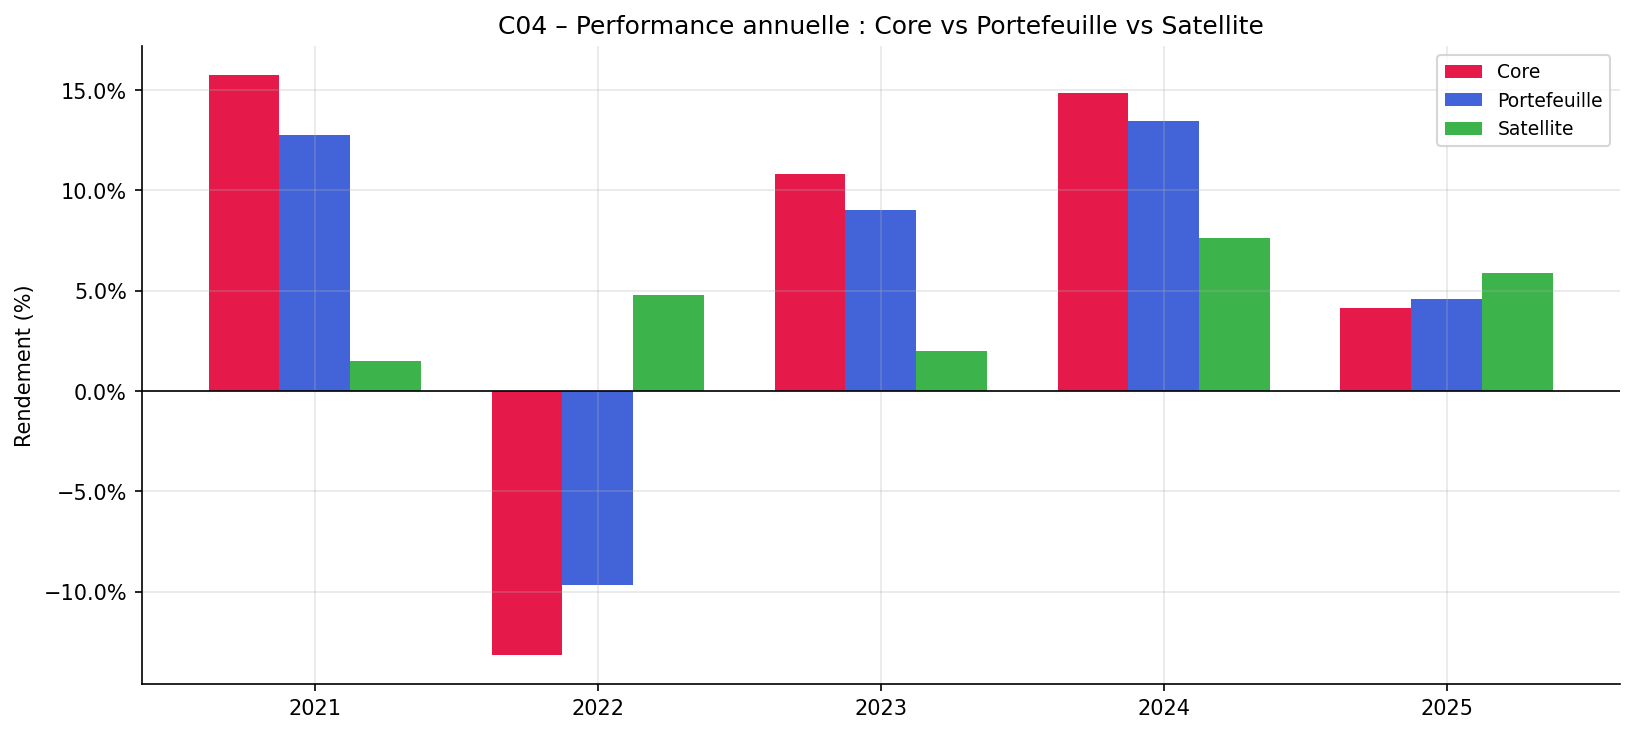
\includegraphics[width=0.9\textwidth]{C04_annual_grouped_bar.png}
    \caption{Décomposition annuelle : Core vs Portefeuille vs Satellite.}
\end{figure}

\begin{figure}[ht]
    \centering
    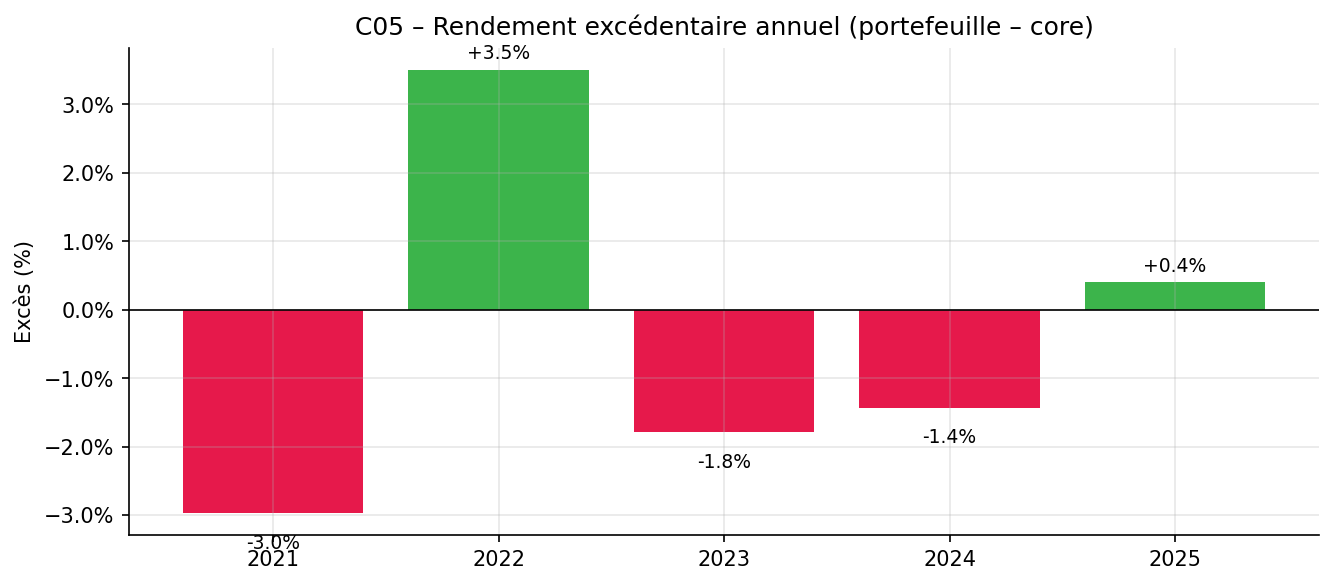
\includegraphics[width=0.9\textwidth]{C05_excess_annual.png}
    \caption{Excès de performance annuel du portefeuille vs Core.}
\end{figure}

Lecture rapide : la Satellite amortit 2022 (choc actions/taux), le portefeuille surperforme alors le Core en relatif, mais reste en léger déficit cumulatif faute de levier et d’un Satellite très prudent. Les contributions annuelles confirment ce profil : meilleure résilience en stress, moindre capture des rallys actions. Couplé à la vol sous-cible (section D04) et au bêta contenu (section D05), cette décomposition plaide pour une V2 avec Satellite un peu plus risquée ou un poids Core/Sat plus flexible.

\section{Diagnostics vol/bêta et attribution par composant}

\begin{figure}[ht]
    \centering
    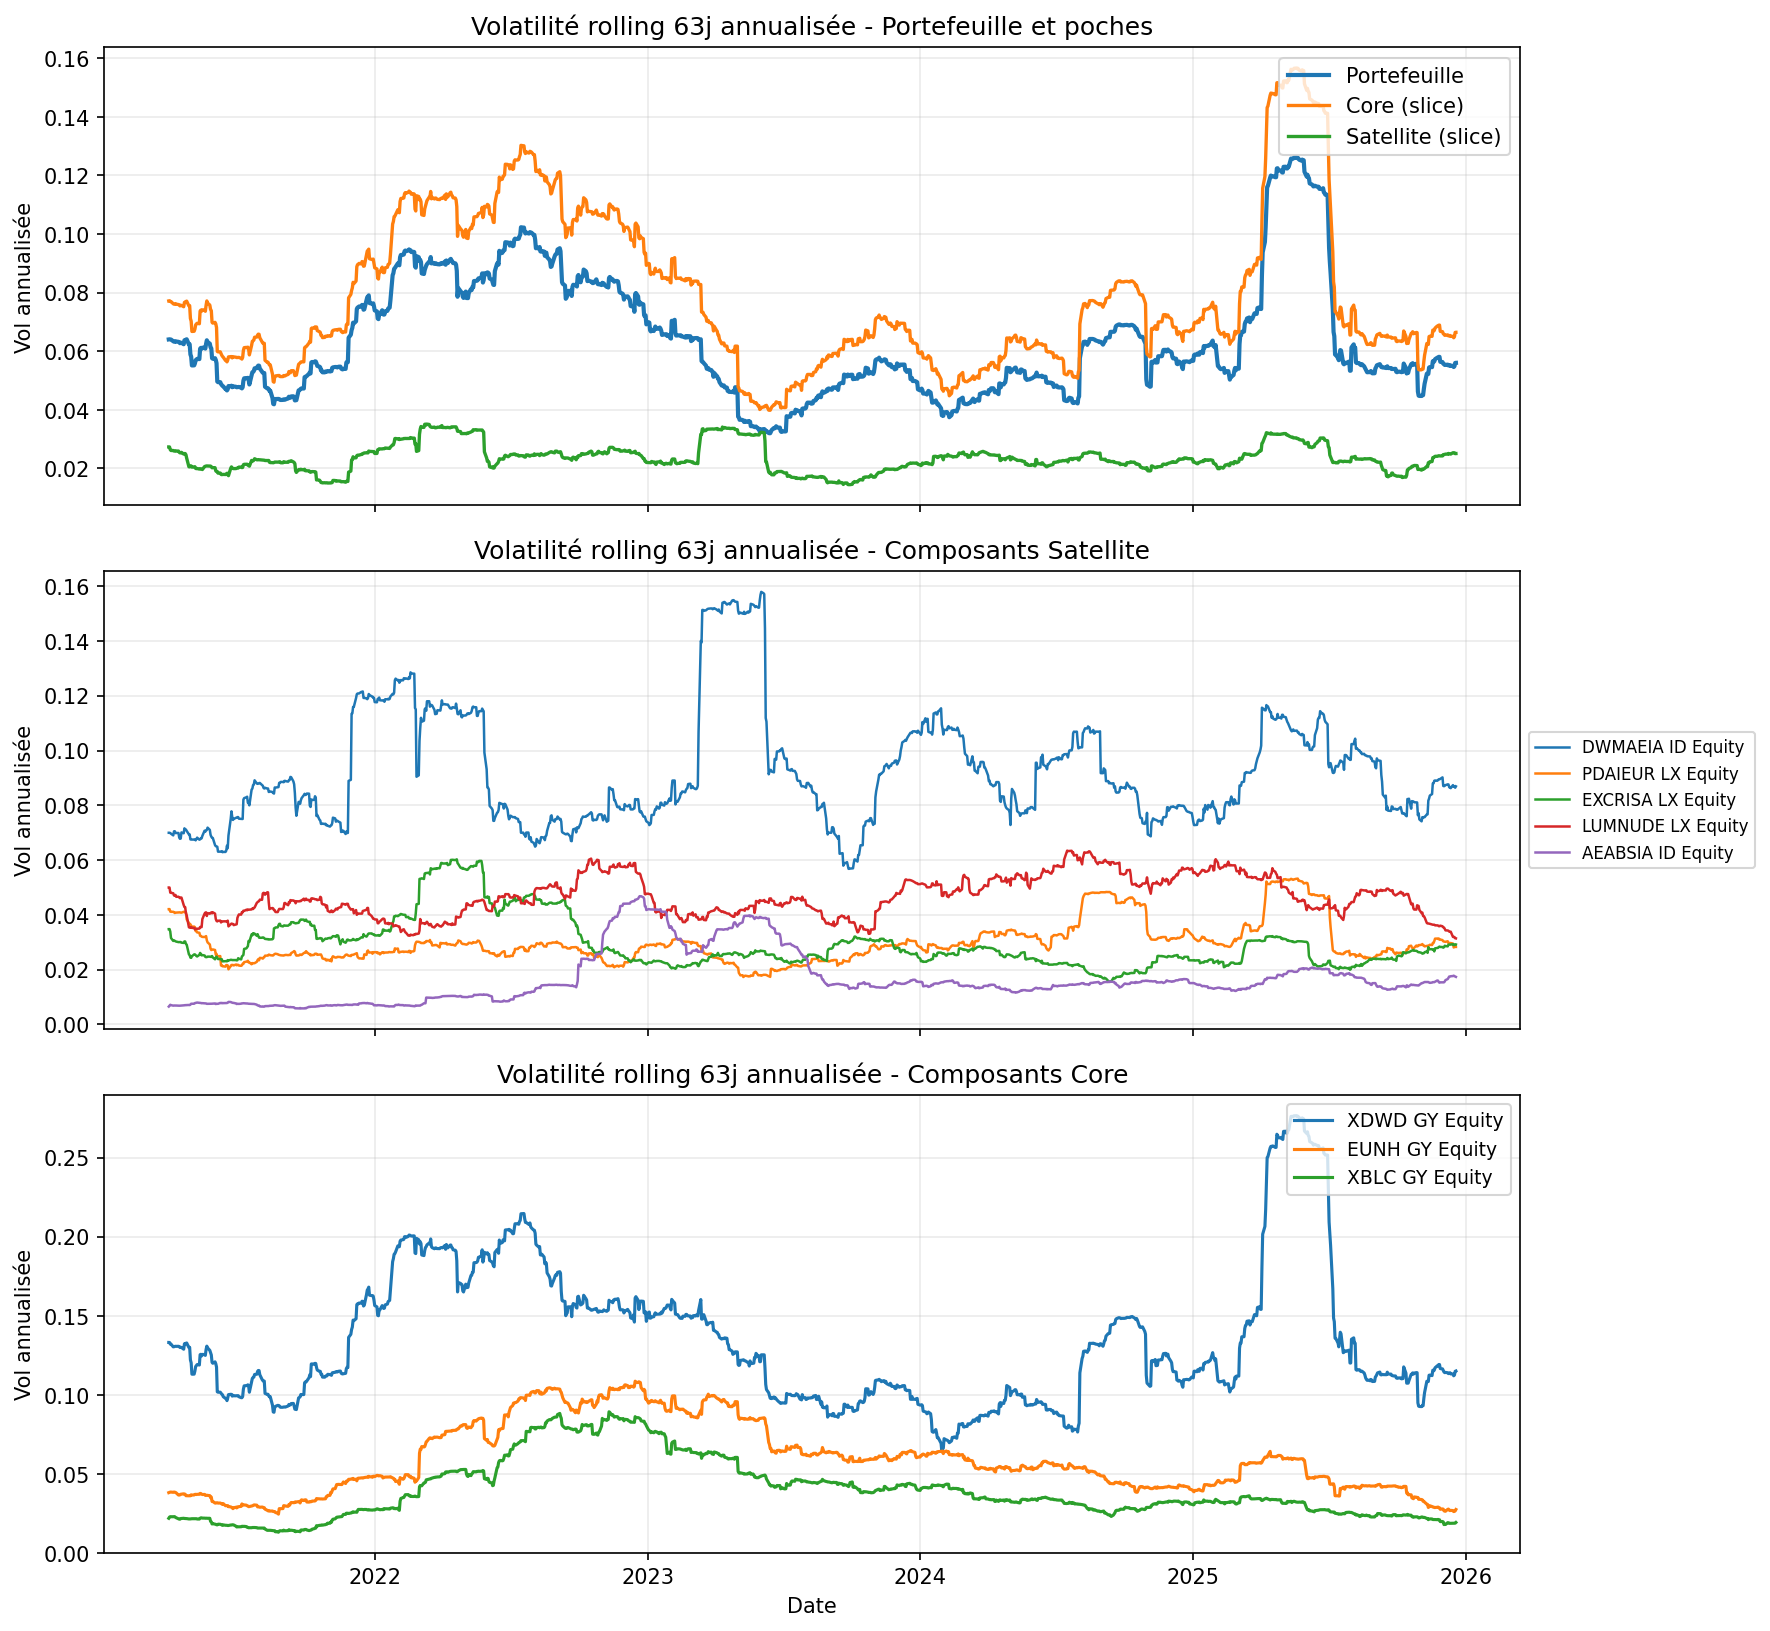
\includegraphics[width=0.95\textwidth]{Z02_vol_rolling_composants.png}
    \caption{Volatilité rolling 63j annualisée : portefeuille, poches et composantes Core/Satellite.}
\end{figure}

\begin{figure}[ht]
    \centering
    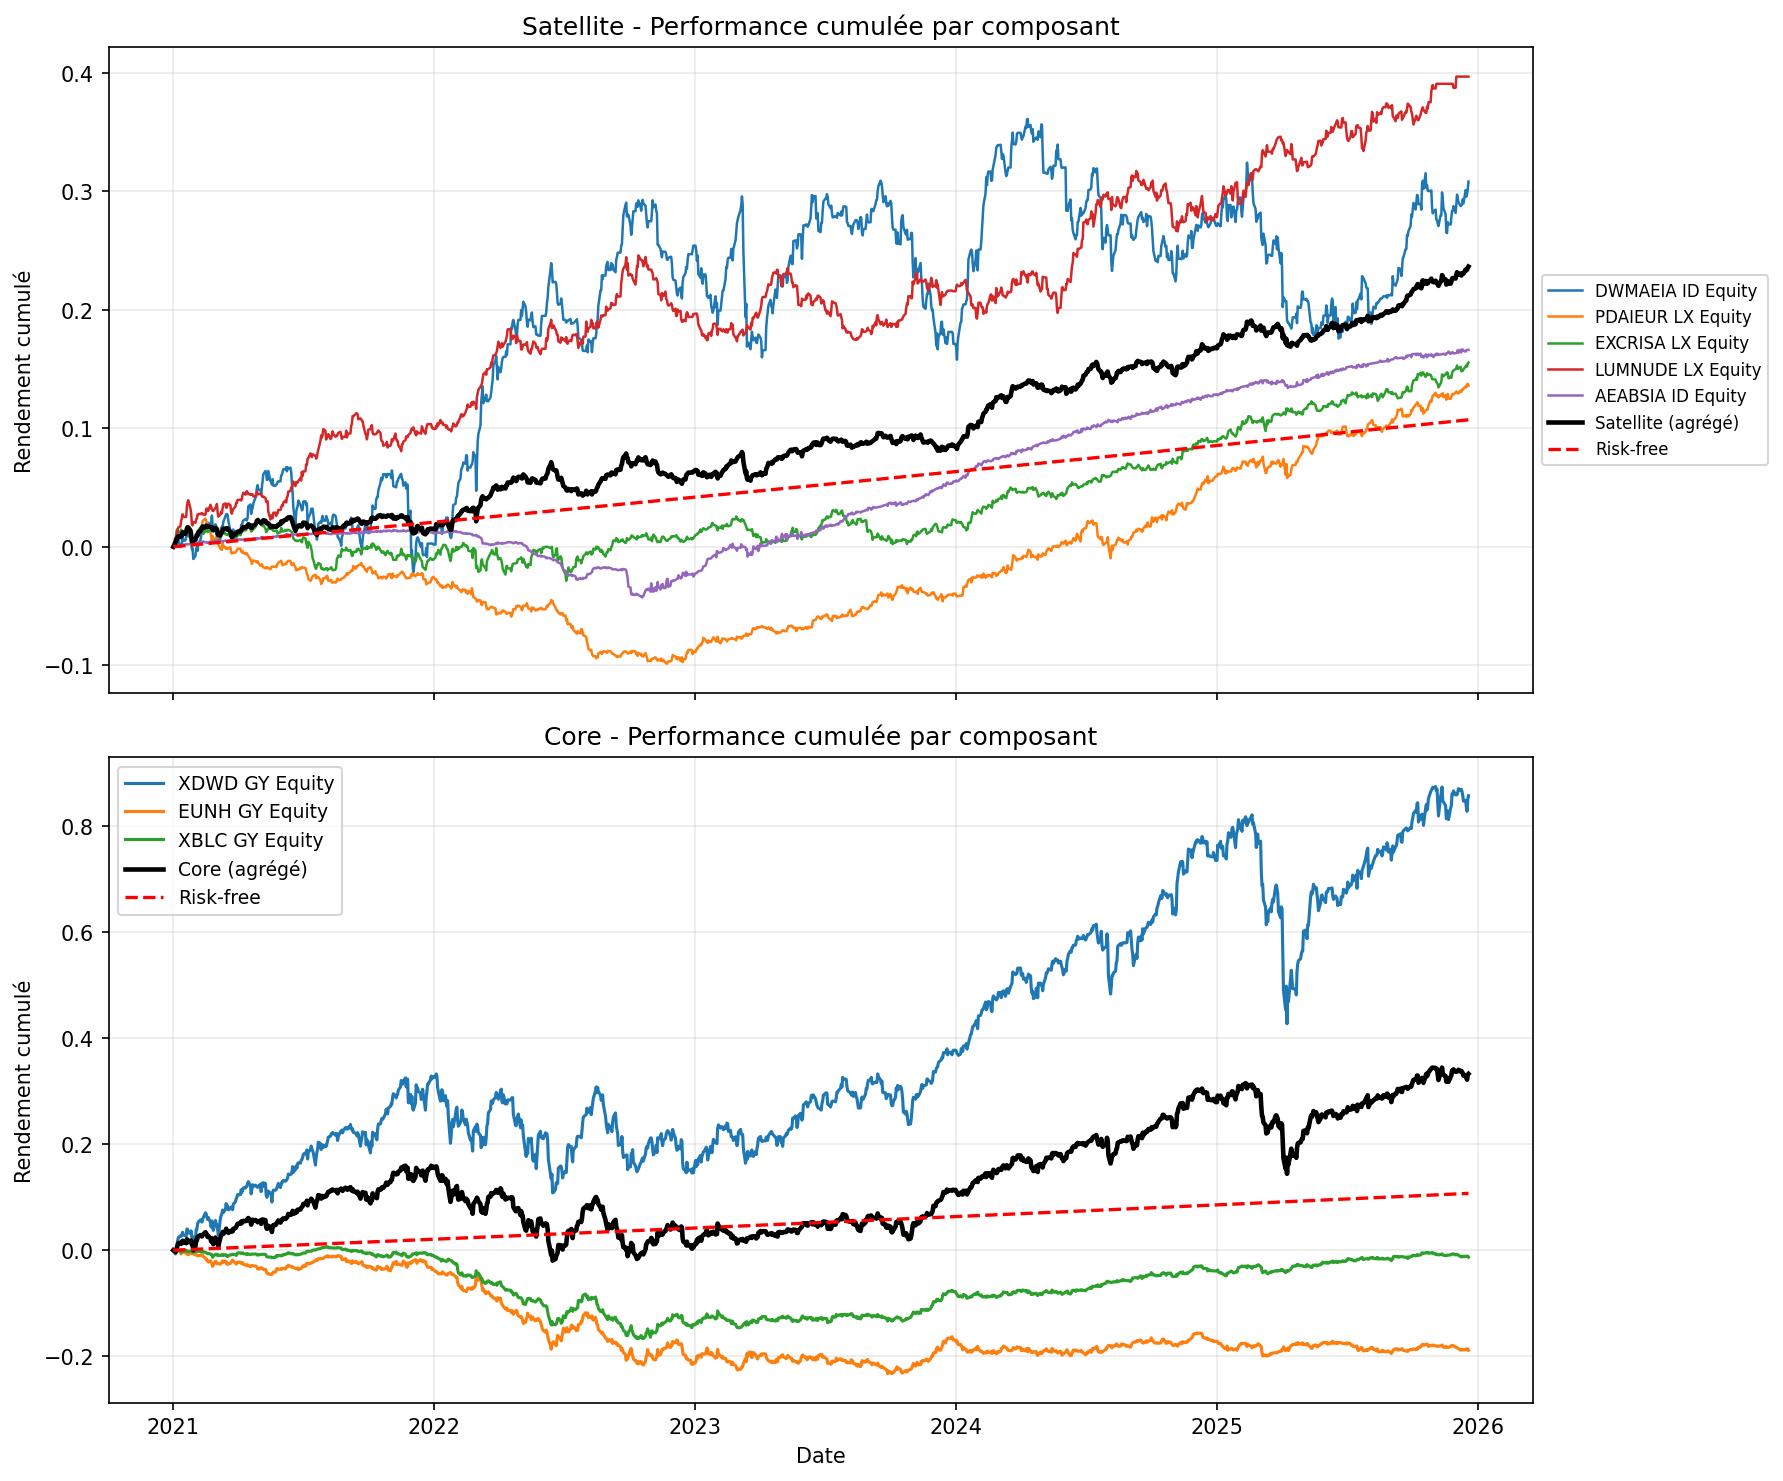
\includegraphics[width=0.95\textwidth]{Z01_perf_composants.png}
    \caption{Performance cumulée par composant (Satellite et Core) avec risk-free (fallback 2\%).}
\end{figure}

\paragraph{Commentaire concis}
\begin{itemize}
    \item Volatilité : la poche Satellite reste autour de 2--3\% annuels, tire la vol du portefeuille sous la borne 8\% hors pics 2025 ; Core domine la volatilité réalisée.
    \item Bêta : les composantes Satellite restent en bêta faible/oscillant autour de 0 (cf. figure D05), cohérent avec la logique de décorrélation first.
    \item Attribution : côté Satellite, DWMAEIA et LUMNUDE portent la majorité de la perf excédentaire vs rf ; côté Core, XDWD domine tandis que EUNH/XBLC restent sous le rf (fallback).
    \item Lecture rf : le rf est plat à 2\% (fallback FRED); remplacer par la courbe Bund réelle affinera les excès sans changer les positions relatives.
\end{itemize}

\paragraph{Note sur rf et sous-performances vs rf}
\begin{itemize}
    \item \textbf{Taux sans risque linéaire} : la série rf est plate car l’appel API Bund (FRED) a échoué ; fallback constant \textbf{2\% annualisé} utilisé (cf. risk\_free.py). Avec l’API ou une série locale Bund, on obtient une courbe quotidienne 10Y.
    \item \textbf{Fonds Satellite sous rf} : PDAIEUR, EXCRISA, AEABSIA. Conservés pour leur bêta/corrélation très bas (décorrélation first). Action possible : passer en réserve si un remplaçant garde $\beta \approx 0$ avec excès $>\,$rf.
    \item \textbf{Core sous rf} : EUNH et XBLC affichent un excès négatif/marginal mais jouent le rôle défensif/rate. Si l’objectif est rendement $>$ rf strict, revoir la sélection Core ou plafonner ces lignes ; sinon on les garde pour diversification et maîtrise de la vol.
\end{itemize}

\end{document}
